\chapter{Autonomous Landing Procedure}\label{chapter:autonomous_landing_procedure}

The implementation of the autonomous landing procedure consisted of two parts. First, the establishment of a sound interface between the autonomy and LSD, ensuring the autonomy's supply of quality information from LSD and the adequate processing thereof. 

Secondly, the adaptive landing behavior itself was implemented.

\section{LSD - Autonomy Interface}\label{subsubsec:lsd_autonomy_interface}

In order to make high quality landing decisions in the autonomy framework one needs high quality information sent to the system by the landing site detection algorithm.

\subsection{LSD Properties}\label{sec:LSproperties}

Before this work the output of the landing site detection algorithm was merely the location of a found landing site. However, as described in \cref{subsubsec:setup:haz_seg} the landing site detection algorithms segments hazards based on roughness and slope. Thereafter, it considers the size of a landing site as well as the uncertainty associated with a certain selected location. 

Simply outputting the location of a landing site is therefore a waste of information when so many characteristics are at hand to make an informed selection. 

I decided on the following properties to be the content of the LSD output:

\begin{itemize}
    \item Location

    The location of the landing site in the world frame.
    \item Uncertainty

    The uncertainty value is also a product of the landing site detection algorithm. It denotes the averaged uncertainty across the area around a given landing site. 
    \item Roughness

    The roughness value the exact value already used for the hazard segmentation step in the landing site detection. See \cref{subsubsec:setup:haz_seg} for an explanation of this property.
    \item Size

    To determine the size of a landing site, the landing site detection algorithm performs a distance transform on the created landing site map in order to find the closest non-landing site for any found landing site. This returns the radius of the largest valid landing circle around a landing site. Calculating the physical value, the metric radius is returned as the size of a landing site.
    \item Obstacle Altitude

    The obstacle altitude was newly introduced in this work. It defines the current highest point of the aggregated DEM's highest resolution layer. As no actual object detection is performed and no hazard information is retained in this visual pipeline, this value serves the autonomy as an indication of the obstacles heights to avoid in the vicinity of a certain landing site. More on this can be read in \cref{subsec:actn_def}.
\end{itemize}

The final landing site detection output is a custom landing site ROS message containing the above-mentioned characteristics of the detected spot. For more detailed explanations of these properties see \cref{subsubsec:setup:aggregation} and \cref{subsubsec:setup:haz_seg}.

Note: The supplied landing site from LSD already underwent a filtering procedure utilizing the roughness, slope, size and uncertainty properties. The value in reconsidering them again in the autonomy is two-fold.

First, we have to remember that LSD does not use the current distance to the drone in its landing site segmentation. Therefore, in order for the autonomy to be able to weight the quality of a landing site (roughness, slope, size, uncertainty) against its convenience (distance to the drone) we need the complete set of properties at all times.

Secondly, a bigger handle in the weighting decision of these properties against each other is desirable. For instance, as mentioned in \citet{LSD2}, the uncertainty values rise significantly in monotonous areas. Thus, a reweighing of the properties is required for optimal performance.

\subsection{Landing Site Heuristic}\label{subsec:heuristics}

\begin{figure}[h]
    \centering
    \includegraphics[scale=0.2]{images/autonomous_landing/new_heuristics.png}
    \caption{Schematic of new properties}
    \label{fig:new_properties}
    \end{figure}

The autonomy processes the in \cref{sec:LSproperties} listed values in order to arrive at the in \cref{fig:new_properties} shown properties:

\begin{itemize}
    \item Current Distance to Drone $L_{dist}$

    Well likely the single most important characteristic of a landing site\footnote[2]{Each received landing site has already undergone a threshold filtering regarding slope and roughness.}. Each iteration the current distance to the drone's position is calculated for each retained landing site. The distance is then normalized by dividing it by the cruise altitude which is 100 m. In practice there were easily enough landing sites found while moving to allow landing sites to fall off when being farther away than 100 m.
    \item Roughness $L_{rough}$

    The roughness property is the unaltered roughness value received from LSD. It is already normalized and enters the loss function as it is. 
    \item Uncertainty $L_{var}$

    The same holds for the uncertainty. It is already normalized by design and enters the loss function unaltered.
    \item Size $L_{size}$

    Analogous to the roughness and uncertainty properties the size comes from the landing site detection directly. However, unlike the two preceding properties it is not normalized but simply denotes the metric radius of the largest circle of valid landing area that can be fit around a given landing site. This is achieved in LSD by performing a distance transform on the created landing site image.

    In order to normalize this value the maximum landing site size is retained and each landing site's size is divided by it in order to achieve normalized size information.

    Also, as can be seen in \cref{eq:loss_fct}, the size contribution enters the loss function with a negative sign. This is due to the fact that compared to all other characteristics, the size defines a property that we would like to maximize.
    \item Verification Altitude $L_{verAlt}$

    A site's verification altitude is the smallest vertical distance between the drone and the landing site at which that site was (re-) detected. 

    The verification altitude is a useful property because of numerous reasons.
    \begin{itemize}
        \item Further Indication of Certainty

        First, similar to the uncertainty metric the verification altitude indicates how certain we can be about a detected landing site as spots detected at lower flight altitudes are more likely correct due to the reduced depth error. Even though it might seem overlapping with the uncertainty property in this regard, these two characteristics are quite complementary as the uncertainty takes OMG convergence and camera specifics into consideration while the verification altitude is a purely location based metric.
        \item Landing Site Property Updates

        As the verification altitude yields a simple and good estimation of the trustworthiness of an incoming landing site, it can be used as a flag to know, when a landing site's properties should be updated. When a landing site is re-detected with a verification altitude lower than the previously stored one, the algorithm trusts it more and alters the previously stored properties to the new ones received.
        \item Verification

        Continuously updating the verification altitude upon re-detection allows us to determine the lowest altitude, at which a landing site was re-detected. This information can be used to verify that a given site was considered a valid landing spot even at low altitudes. 
    \end{itemize}
\end{itemize}

The final heuristic defining the quality of a landing site is in fact a square loss function:

\begin{equation}
    L_{LS} = w_{dist}L_{dist} + w_{rough}L_{rough} + w_{var}L_{var} + w_{size}L_{size} + w_{verAlt}L_{verAlt}
    \label{eq:loss_fct}
\end{equation}


\subsection{Landing Site Manager}

Prior to this thesis, the landing site manager received artificially generated landing sites from a dummy landing site node. In this work the LSM was connected to the actual landing site detection output. See \cref{subsubsec:LSM} for an introduction of the landing site manager.

With the new landing site properties introduced in \cref{subsec:heuristics} the metric according to which a landing site is evaluated is no longer a maximizing heuristic but a loss function to be minimized. Therefore, the simple switch of a min-heap to a max-heap was done to efficiently consistently switch the worst landing site and order the incoming one.

Apart from the new heuristics and the handling thereof, the following important new concepts were introduced for the landing site manager:

\subsubsection{Re-Detection}\label{subsubsec:redetection}

In the LSM's state before this thesis, each landing site was considered individually and processed. The worst landing site according to the heuristic was filtered out, and the new landing site was put in its place and then ordered into the min heap.

Re-detection defines the mechanism of assessing the proximity of an incoming landing site to the already considered landing sites in the buffer. If an incoming landing site is close enough to a previously detected site, this is considered a re-detection. In that case, the new landing site is not entered into the buffer but instead, the previously detected landing site has its properties updated.

However, this property update is only performed, when the incoming landing site's was detected at a lower flight altitude. Expressed in specific terms this means, that the landing site is only updated if the incoming landing site's verification altitude is lower than the previously detected one. This is because, more trust is placed onto landing sites detected at a closer distance to the ground. 

The benefit of the update of the characteristics lies in the refinement of the site's information and therefore the retention of a higher quality landing site candidate.

The proximity within which an incoming site is considered a re-detection of another is determined by a linear interpolation. At 100 m altitude any landing site within a 1 m distance to another is considered the same site. At the verification altitude which was set to 2.5 m during this work, the re-detection distance is 0.1 m. This change of threshold implicitly accounts for the larger terrain errors made at higher altitudes. 

The schematic re-detection procedure is shown in \cref{fig:ls_redetection}.

\begin{figure}[h]
\centering
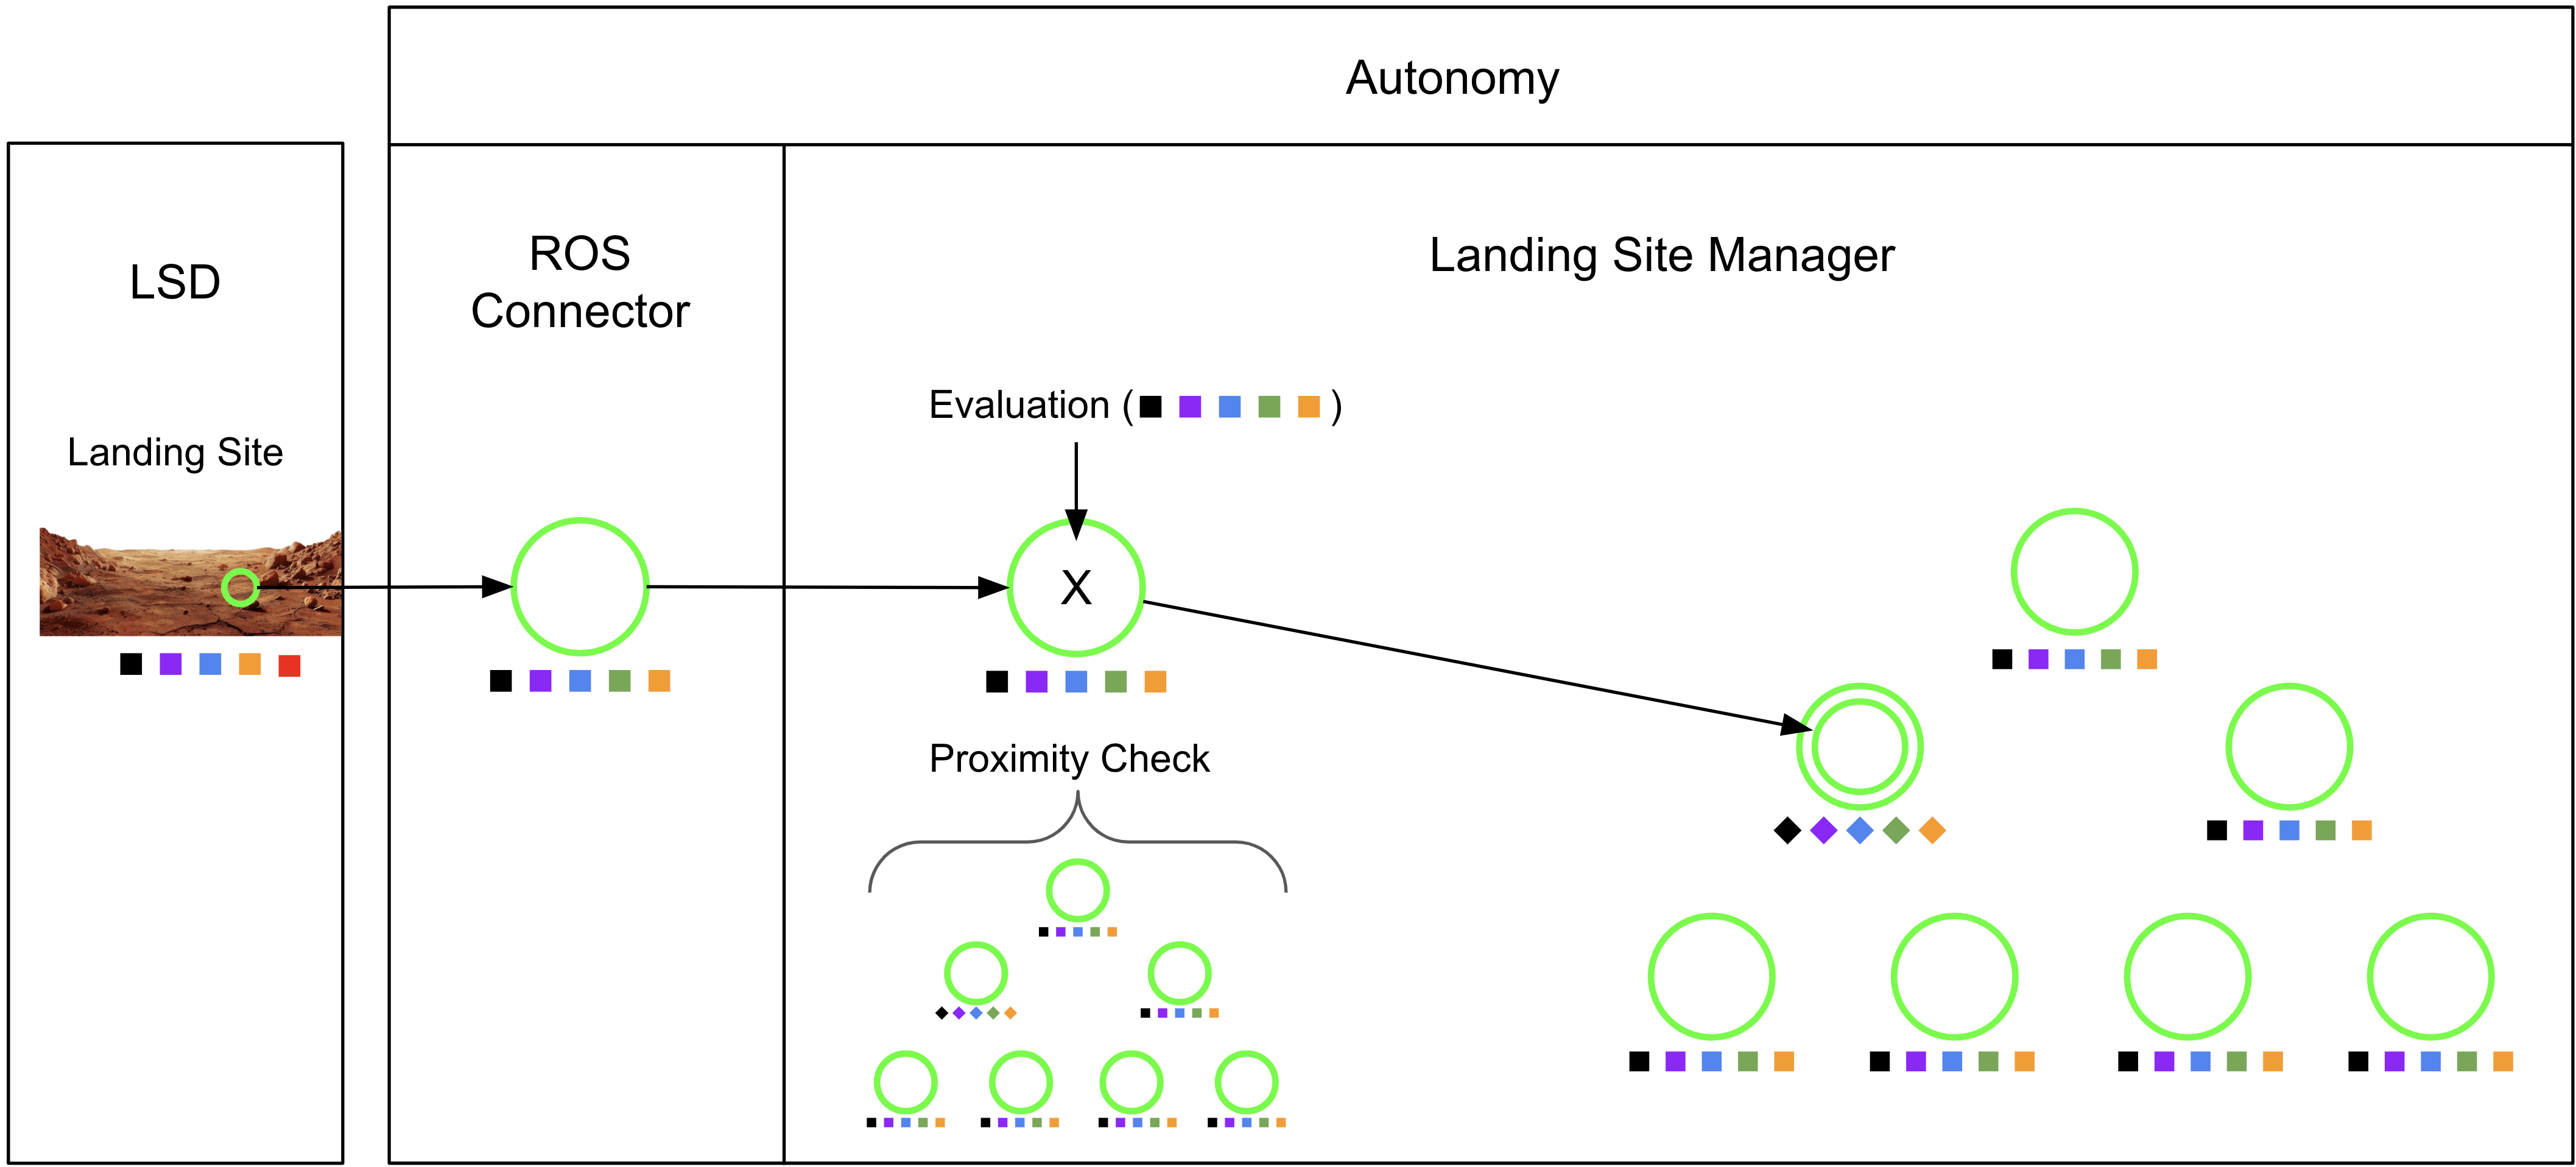
\includegraphics[scale=0.16]{images/autonomous_landing/re-detection.png}
\caption{LS re-detection: When the proximity check is successful, the incoming landing site updates an existing landing site instead of entering the buffer itself.}
\label{fig:ls_redetection}
\end{figure}

The new heuristics are indicated with the colored squares according to their introduction in \cref{fig:new_properties}. Note that the obstacle altitude property is part of the LSD output but as it is not part of the loss function, it is not considered in the LSM's ordering. Secondly, the verification altitude like the distance to the drone are derived and attached in the ROS connector.

\subsubsection{Selection}

In the already existing autonomy framework, the landing site handling was very similar. Landing sites were ordered, and upon entering the landing state, the best one is shared with the navigation nodes through the blackboard variable interface. The selection happened therefore only in the signaling of the landing site manager to the other nodes which landing site to navigate towards.

The landing site manager was changed in this regard to actively choose a landing site and update it consistently. This way, a handle to the current candidate exists. This handle is used for numerous benefits including consistently updating the landing site upon receiving new information, verifying that exact landing site and banning it in case of a verification failure. 

\subsubsection{Verification}\label{subsubsec:verification}

As explained in \cref{subsubsec:redetection}, when a landing site is re-detected, all properties are updated if and only if the verification altitude is lower than previously perceived. This results in a landing site always retaining the lowest altitude at which it was detected.

This promotes the choice of a landing site detected at low altitudes as mentioned in \cref{subsec:heuristics}. What's more, we can use this as a verification tool.

When pursuing a landing site which was detected at 100 m altitude, we need to validate it at a low altitude before committing to it and landing. We can do so safely as, yes, the initial landing site estimate from 100 m altitude might not be a good choice, however as can be seen in \cref{eq:SFM_depth_error}, given an approximate baseline of 15 m at 100 m altitude with a focal length of 256 and an assumed subpixel disparity error of 0.5, the structure from motion algorithm yields depth measurements with an approximate depth error of 1.3 m. Therefore, when verifying a landing site at about 2.5 m altitude, the drone has sufficient buffer to potential terrain.

Thus, the verification consists of the low altitude hovering above a landing site, consistently scanning the terrain using the stereo camera which constantly sends landing sites to the autonomy. After a verification timeout duration is reached, the verification altitude of the chosen landing site is compared to the hover altitude and if they are within a small error threshold of each other, the site is considered verified and landing is initiated.

If the verification fails, the chosen landing site has to be banned. This includes not only the removal of the landing site from the buffer, as it might be re-detected in the future. Instead, the landing site has to be entered into a ban list against which new landing sites are compared and if a re-detection of an incoming landing site with a banned one is triggered, the incoming landing site is ignored. 

The reason for this mechanism lies in the exclusion of the possibility of repeatedly detecting and pursuing promising false candidate.

The final procedure is shown below in \cref{fig:lsm_complete}. A received landing site is checked regarding its proximity to the selected landing site, the banned landing sites and the current landing sites in the buffer. If it is close enough to one of these sites, it is discarded in the case of the ban list and otherwise used for re-detection. If it's not the case, the landing site is entered into the LS buffer, as shown in \cref{fig:lsm_ls_processing}.

\begin{figure}[h]
\centering
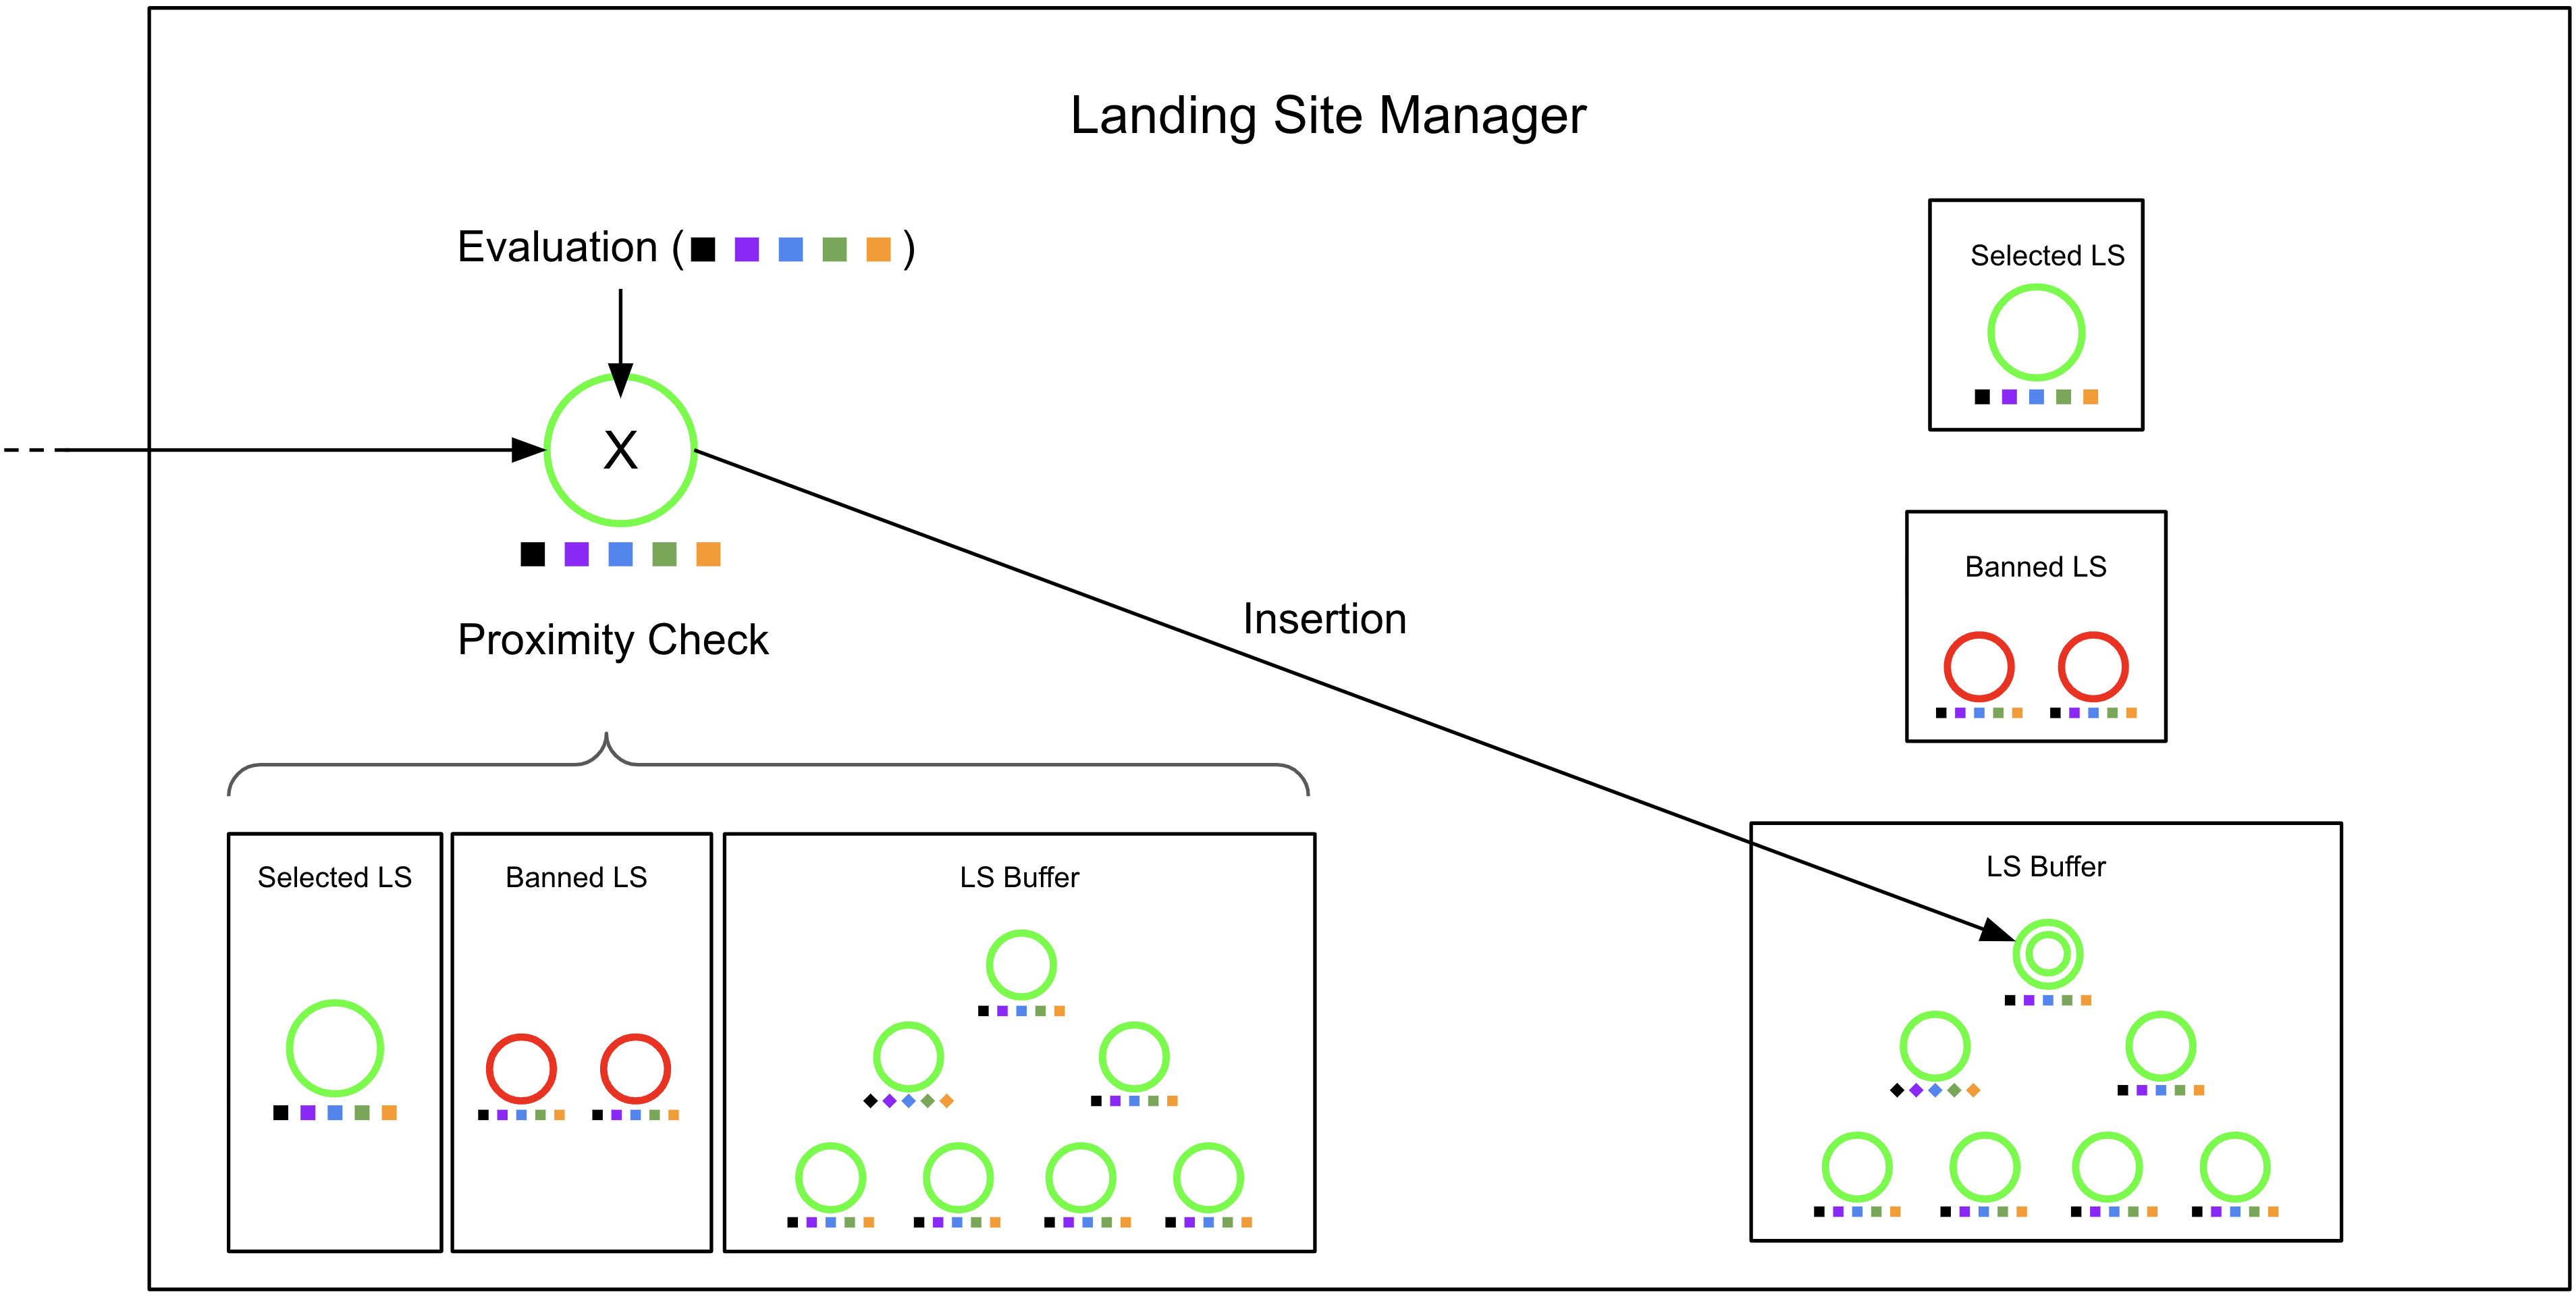
\includegraphics[scale=0.2]{images/autonomous_landing/lsm_complete.png}
\caption{Complete LSM landing site handling}
\label{fig:lsm_complete}
\end{figure}

\section{Conceptual Behavior}\label{sec:concept_beh}

To understand the landing behavior, the mission as a whole has to be considered.

\subsection{General Mission}

Looking at a mission performed by the autonomy framework at a high level and laying emphasis on the landing pipeline, the procedure looks like this:

\begin{itemize}
    \item Preparation
    
        \begin{itemize}
            \item Beforehand, a mission is created manually by exporting a QGC plan and converting it to the format readable by the autonomy.
            \item The configuration parameters are set to the adequate values for the flight at hand.
            \item The autonomy is started.
            \item The necessary connectors with the ROS nodes, the flight controller and further auxiliary nodes are initialized.
            \item An actuator check is performed.
            \item Finally, the final starting signal is awaited.
        \end{itemize}
        

    \item Takeoff
    
    The drone takes off vertically until the desired course altitude of the first entered waypoint is reached. During this vertical flight stereo starts off and detects point clouds which are given to LSD for the map aggregation and landing site segmentation. After reaching the switching threshold mentioned in \cref{subsec:switching}, stereo is deactivated and SFM starts up. However, as the rotorcraft is still in mere vertical motion, no point clouds are created by SFM.

    \item Mission

    Upon reaching the first waypoint's altitude, the drone starts lateral motion. This is where SFM starts supplying LSD with the first non-trivial landing sites which are transferred to and processed by the autonomy. The mission may have numerous waypoints and upon reaching the last one, the landing sequence is initiated.

    \item Landing
    
    The landing behavior uses the perceived landing sites in order to reactively and safely determine, validate and approach a landing site. When the landing decisions have concluded, the drone lands aka it descends until ground contact is established. The decision-making is explained in detail in \cref{subsec:landing_behavior}. 

    \item Termination

    Upon having successfully landed, the drone enters the termination state which cleans up the autonomy pipeline and disarms the drone. Given that the drone's battery has a sufficient residual voltage, a new mission can be started.
\end{itemize}

\subsection{Landing Behavior}\label{subsec:landing_behavior}

The core of the landing behavior is what happens between selecting a landing site and finally vertically landing. As previously mentioned, the landing behavior was designed to be safe. Additionally, within this safe behavior space, the effort was made to derive an efficient behavior implementation.

The conceptual landing behavior which is started at the end of the mission state and repeated a predetermined number of times is the following:

\begin{enumerate}
    \item A check is made, whether any landing sites have been registered yet
    \begin{enumerate}
        \item If no landing site was detected, go to a new location and fly a pattern until a potential site has been found.

        This procedure is repeated a predetermined amount of times. If they fail consistently, the drone returns home by ascending to a safe altitude, traversing to the home location and descending until touchdown, slowing down upon reaching a certain proximity above ground.
        \item If there are landing sites, order them in ascending order (regarding their loss scores) and pick the best one.
    \end{enumerate}
    \item Using the drone's current position, the landing site's location and the site's obstacle altitude parameter, determine a minimum safe clearing altitude up to which to ascend.
    \item Traverse to the considered landing site.
    \item Descend to a predetermined verification altitude above ground (during this descent the stereo camera takes over at some point).
    \item Hover for a given duration.
    \item Perform the verification check introduced in \cref{subsubsec:verification}.
    \begin{enumerate}
        \item If verification is successful, initiate landing.
        \item If verification failed, ban landing site and return to point 1.
    \end{enumerate}
\end{enumerate}

\section{Software Implementation}\label{sec:landing_impl}

The final landing behavior is implemented in the form of a behavior tree which allows the adaptive and scalable implementation of simple tasks to create a larger and more complex decision-making entity.

\subsection{Action Definition}\label{subsec:actn_def}

The autonomy framework already defined the core control flow nodes as well as some action nodes required for the landing behavior. These are introduced in \cref{subsec:setup:behavior_tree}. Hereafter displayed is a list of additionally required actions for the landing behavior. It should be noted, that they define individual, independent actions and should not be considered a description of the entire behavior. For this consider \cref{subsec:behavior_tree}

\begin{itemize}
    \item CheckLandingSiteAction

    Simple utility action which checks whether any landing sites have been found by querying the LSM's landing site buffer length.
    \item ChangeAltitudeLSAction

    This action was implemented with the purpose to allow us to vertically move to a certain fixed altitude above a chosen landing site. This allows the drone to easily get to a predefined safe altitude at which it traverses to a found landing site.
    \item GetLandingSiteAction

    Upon leaving the mission state and entering the landing state, the autonomy attempts to select the currently best landing site according to the in \cref{subsubsec:LandingSiteHeuristic} introduced loss function.

    This is done by using the landing site manager in order to rank the landing sites in an ascending sorted list (as opposed to a max-heap) and selecting the first entry with the lowest loss.

    The selected landing site is then stored in a blackboard interface which allows easy data sharing between all the actions within the autonomy.

    Once a landing site has been chosen, the fail-safe mechanism to go to that landing site is the following:

    \begin{enumerate}
        \item Ascend to a safe altitude.
        \item Traverse laterally to the landing site's position.
        \item Descend to the landing site or verification altitude.
    \end{enumerate}

    The question remains however, what the adequate clearing altitude is. The goal is to find an altitude high enough to fly safely without the risk of collision yet low enough as to not waste energy for the increased ascent / descent distances.

    This is where the aforementioned obstacle altitude from \cref{subsec:obstacle_altitude} comes in. The obstacle altitude gives us an indication of the height to clear around the landing site. Therefore, we can take this as the start altitude for the derivation.

    As the DEM created by LSD covers only a limited area, the obstacle altitude is only an indication of the highest terrain present at the chosen landing site. The worst case scenario would be the detection of the landing site at the very edge of the DEM shortly before significantly higher terrain starts. Therefore, one has to anticipate this case. 

    In practice a safe altitude buffer is implemented by assuming the worst case 45-degree incline of the terrain starting immediately at the landing site. Thus, the necessary clearing altitude can be derived by linearly interpolating the final value from the initial obstacle altitude and the distance between the drone and the landing site which needs to be covered.

    In the end to not ascend to excessive heights, the clearing altitude is capped at a pre-determined, terrain-based fail-safe altitude

    \begin{align}
        z_{\text{clear}} &= z_{\text{obst.}} + z_{\text{buffer}} + d_{\text{drone-LS}}\\
        z_{\text{clear}} &= \text{min}\left(z_{\text{clear}}, z_{\text{fail-safe}}\right)
    \end{align}
    Above we can see the derivation of the clearing altitude where $z_{\text{clear}}$ defines the clearing altitude, $z_{\text{buffer}}$ a safety buffer on top of the obstacle altitude, $d_{\text{drone-LS}}$ the drone's current distance to the site and $z_{\text{fail-safe}}$ the fail-safe altitude at which the clearing altitude is capped. A schematic visualization of this is depicted in \cref{fig:clear_alt}.
    \item LandingSiteVerificationAction
    
    Once a landing site is chosen, we have to make sure it's a good spot to land before attempting to do so. 

    The LandingSiteVerificationAction does this by using the verification altitude property of a given landing site:

    When a landing site is detected by SFM at 100 m altitude it will be overwritten when re-detected at 2.5 m above the ground. 

    This is the mechanism exploited in order to verify a landing site. The drone hovers above the landing site for a pre-determined duration in place and attempts to re-detect the chosen landing site. This means that the LSM continuously processing incoming landing sites and if one is close enough to an existing one, it is considered a re-detection. In that case, the landing site is verified, and the landing action can be triggered.

    In case of verification failure, the landing site is not only removed but actively banned in order to prevent future false positives at high altitudes.

    Additionally, as previously mentioned, the verification hovering at low altitudes leads most probably to the detection of close by landing sites. This is arguably as important as the verification of a previous landing site as it yields a good candidate in close proximity. In practice, it turned out,  it is equally likely to verify a landing site as it is to not verify one but detect a high quality landing site close by.
    \item LandingSiteSearchAction

    The previously described actions are core implementations of the nominal behavior in the landing sequence. However, what happens when no landing sites are found, either through fault of the landing site detection setup or due to really unfavorable terrain?

    The most intuitive answer seems a good idea - simply look further for a site. The technical implementation of this task at high altitudes requires the detection by SFM and therefore lateral motion. So an easy solution is to fly a pattern at a new location with the exact same landing site handling procedure as in the nominal case.

    The LandingSiteSearchAction implements this through a predefined rectangle of waypoints which are flown through. This sub-mission is cancelled upon detecting a single landing site. In that case the usual landing procedure is continued.
    \item GetNextPatternCenterWPAction

    In case of failure when looking for additional landing sites, the adaptive procedure is to simply move to a new location and try anew. 

    The drone picks a random position around the final mission waypoint, flies there and again moves laterally in a rectangle shape in the hope of detecting landing sites.

    Note: In case that this action and the subsequent landing site search fail to detect any landing sites, they are repeated as often as the battery state permits it and the drone has to return to the home position.
    \end{itemize}

    \begin{figure}[h]
    \centering
    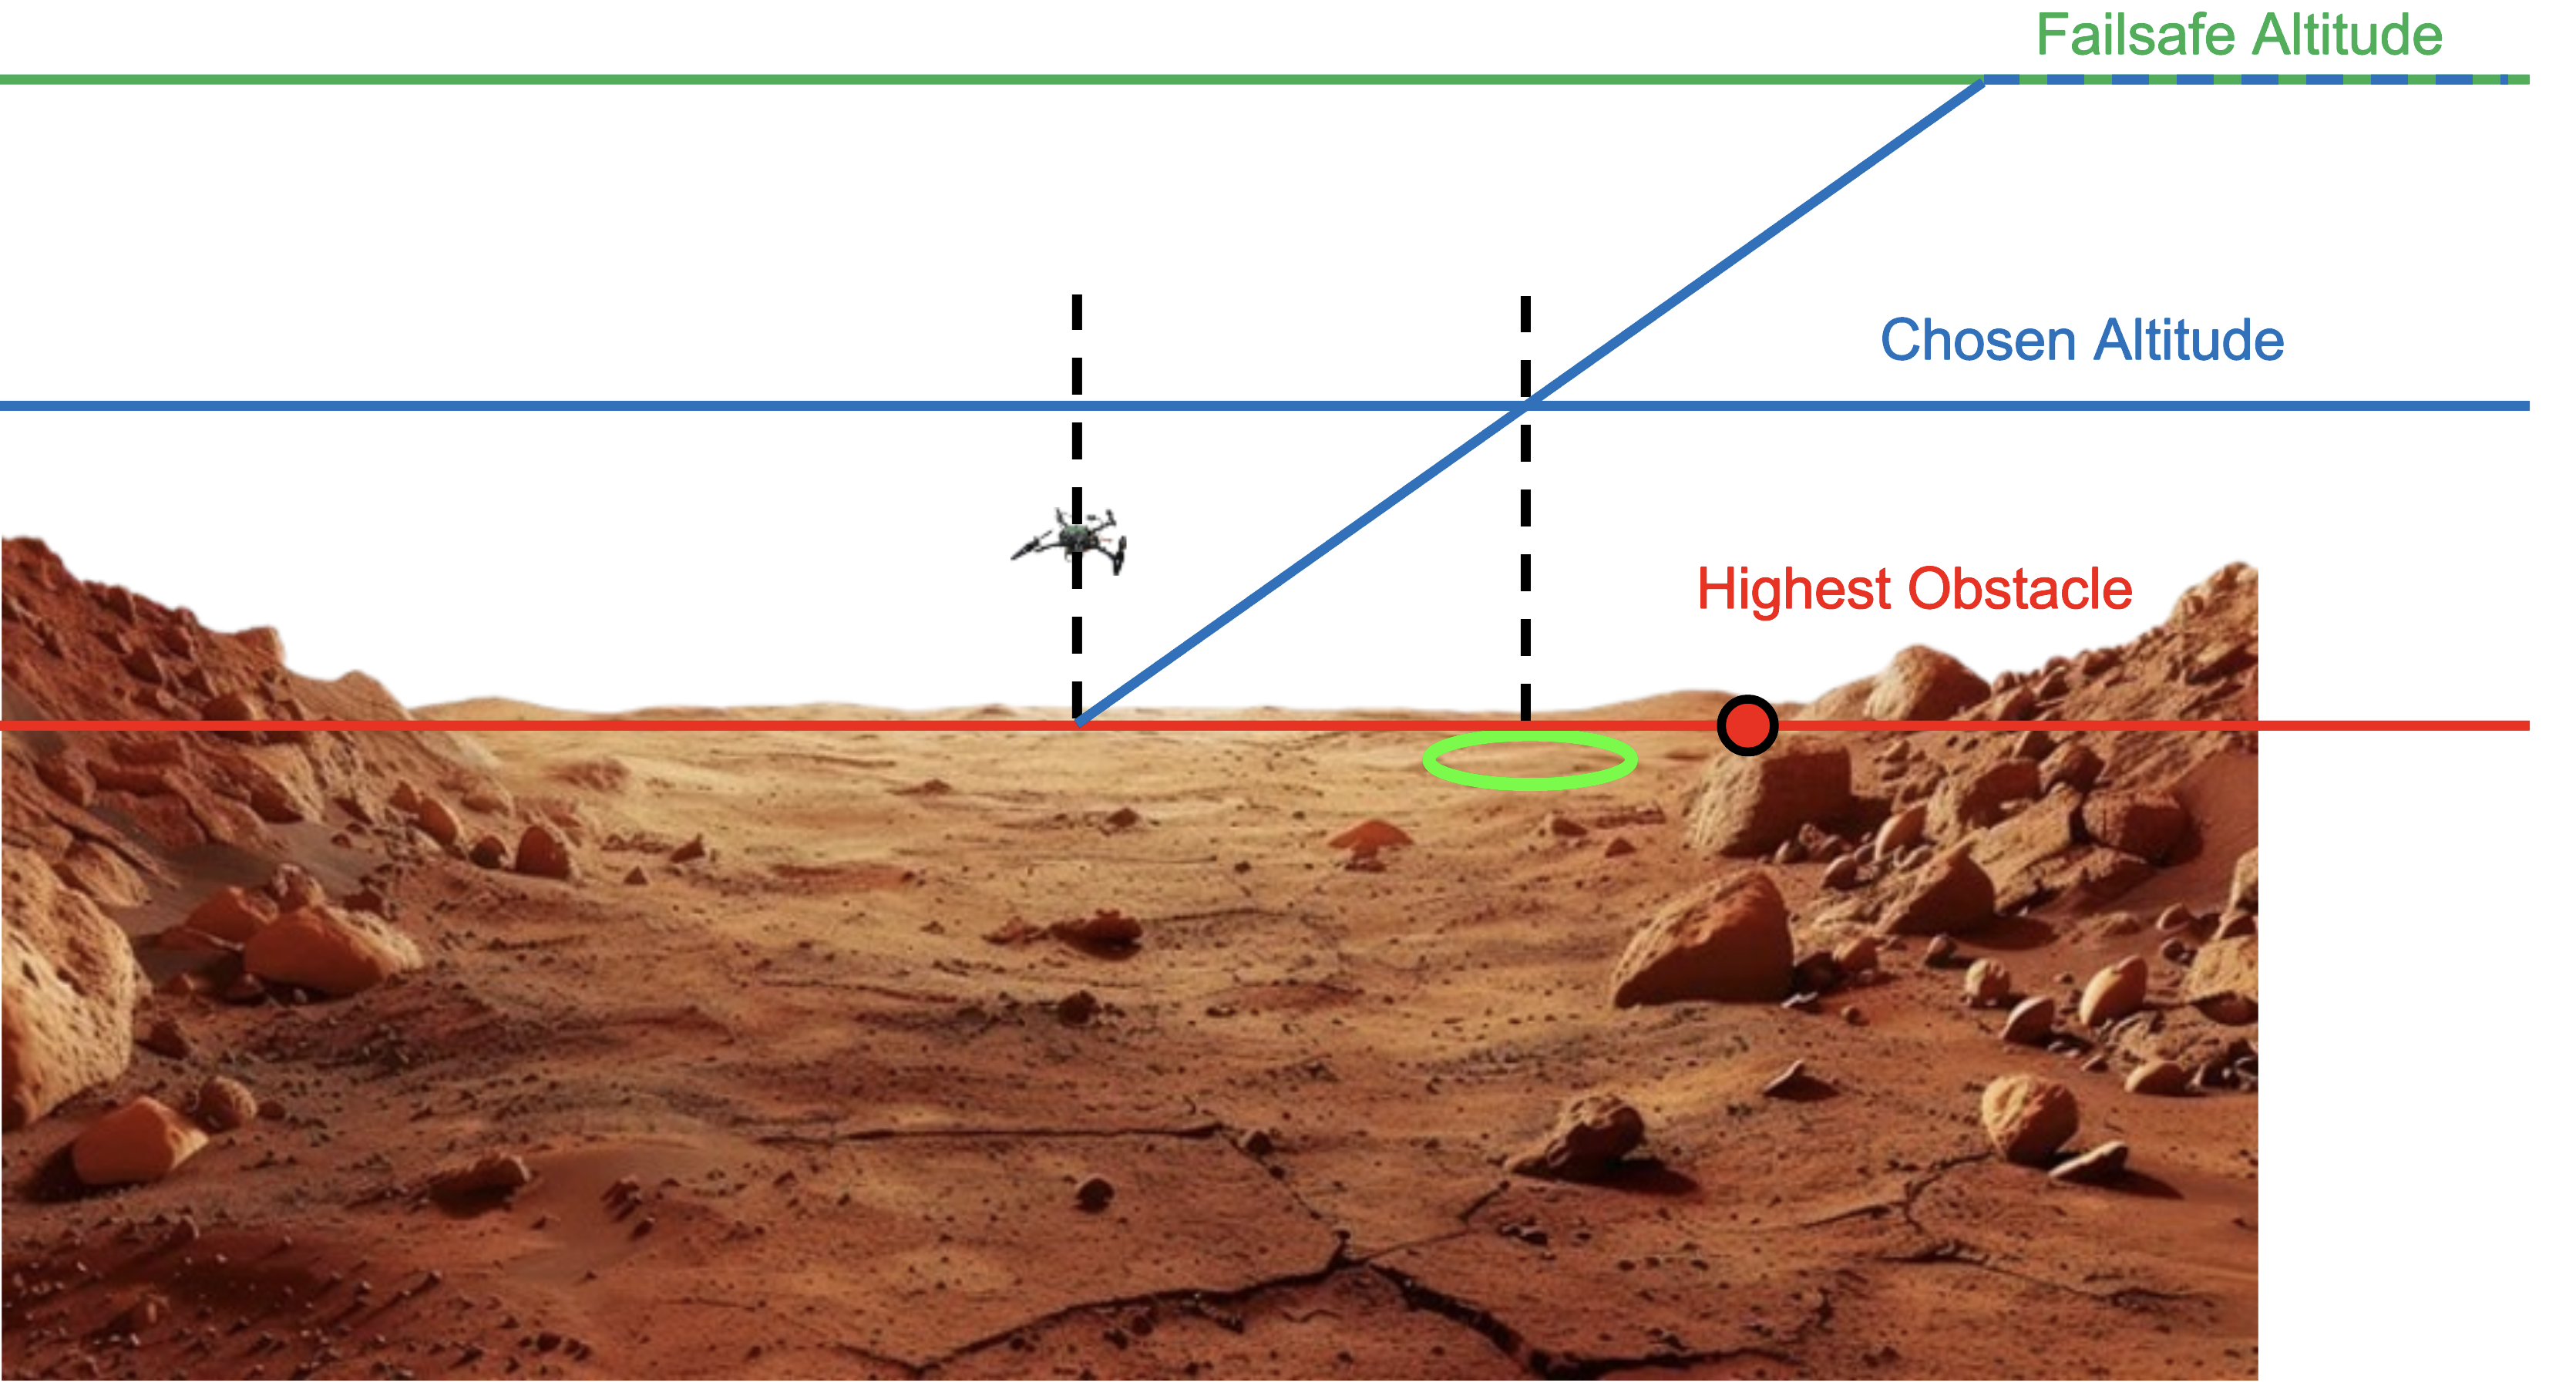
\includegraphics[scale=0.2]{images/autonomous_landing/clearing_altitude.png}
    \caption{Schematic of the clearing altitude decision procedure}
    \label{fig:clear_alt}
    \end{figure}

\subsection{Behavior Tree Implementation}\label{subsec:behavior_tree}

In the following, the behavior tree visualizations follow the scheme introduced in \cref{subsubsec:BT_exp}.

\subsubsection{High Level Behavior}

To improve the readability, first, the high level landing behavior is shown in \cref{fig:high_lvl_bt}:

\begin{figure}[h]
\centering
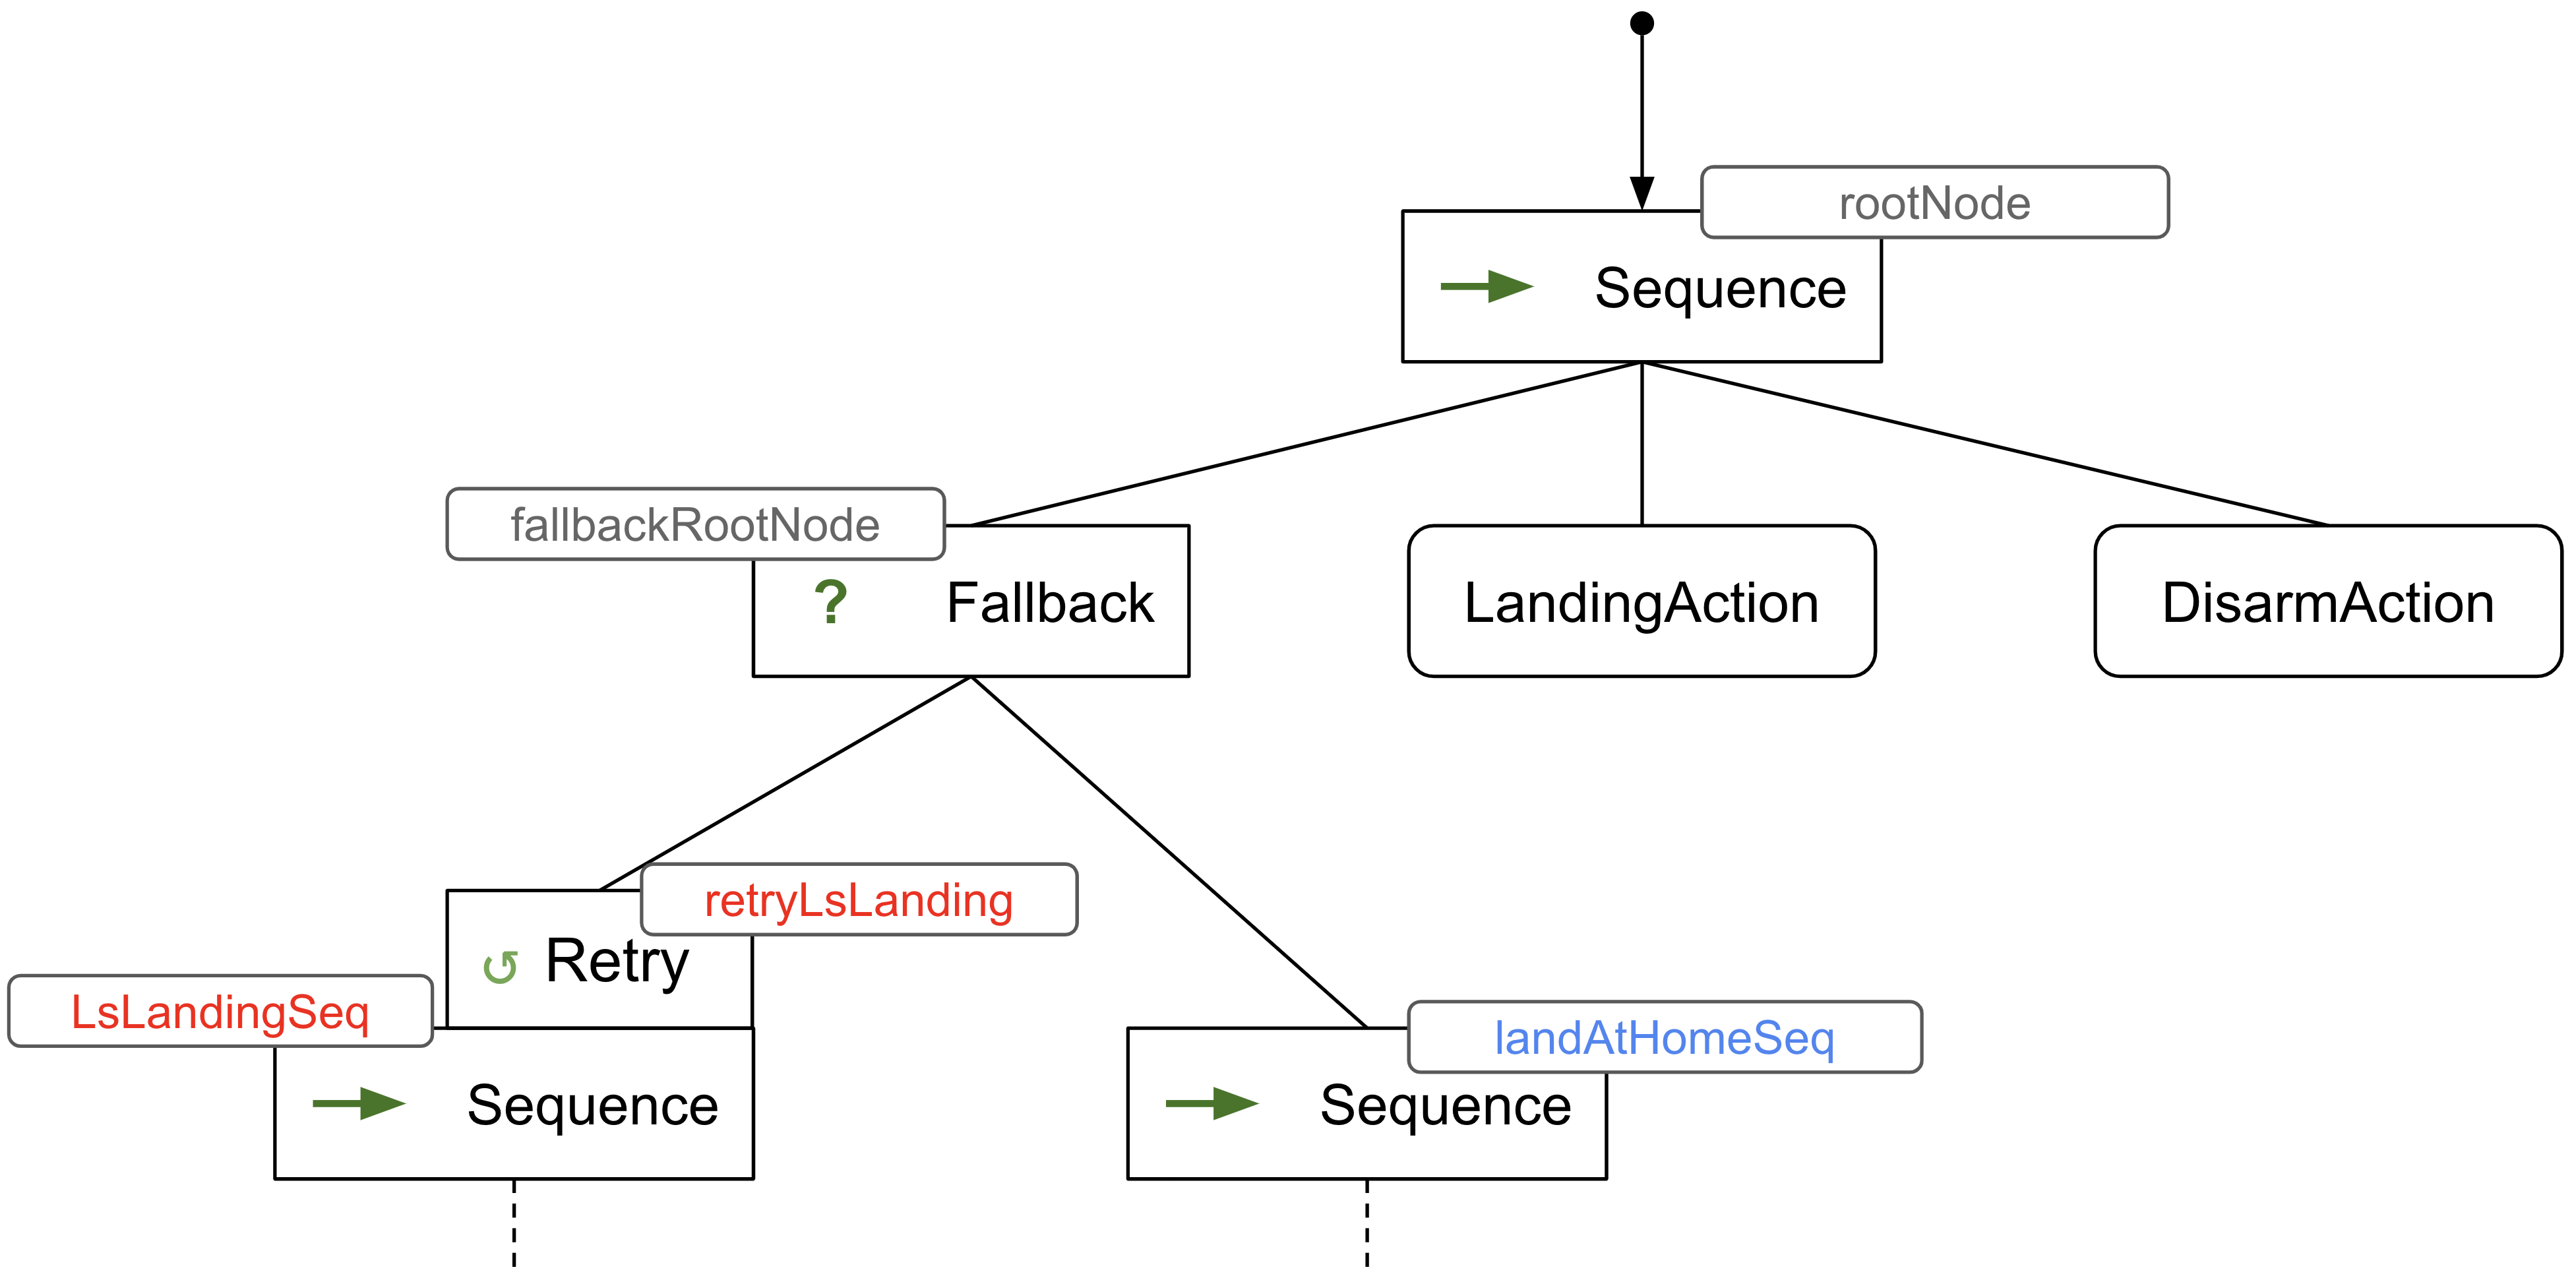
\includegraphics[scale=0.18]{images/autonomous_landing/high_level_BT.png}
\caption{High level landing behavior represented as BT}
\label{fig:high_lvl_bt}
\end{figure}

When the landing state is entered, the root node is initiated. First, the core landing behavior outlined in \cref{subsec:landing_behavior} is attempted repeatedly using the retry decorator node. If it is successful, the fallbackRootNode returns success and the landing Action as well as the disarmAction are executed. If the node fails a certain number of times, it returns the failure state and the sequence node to land at the home position is initiated.

\subsubsection{Core Landing Behavior utilizing Landing Sites}

The conceptual implementation of \cref{sec:concept_beh} is shown in \cref{fig:landing_BT}. As for the behavior tree example from the system overview in \cref{subsubsec:BT_exp}, node names are attached when a node type is used more than once. Due to a lack of space and to improve readability, the action nodes in the VerBehSeq (aka verification behavior sequence) were placed onto two lines. Their order is to be read according to the line connections from the sequence node left to right.

\begin{figure}[h]
\centering
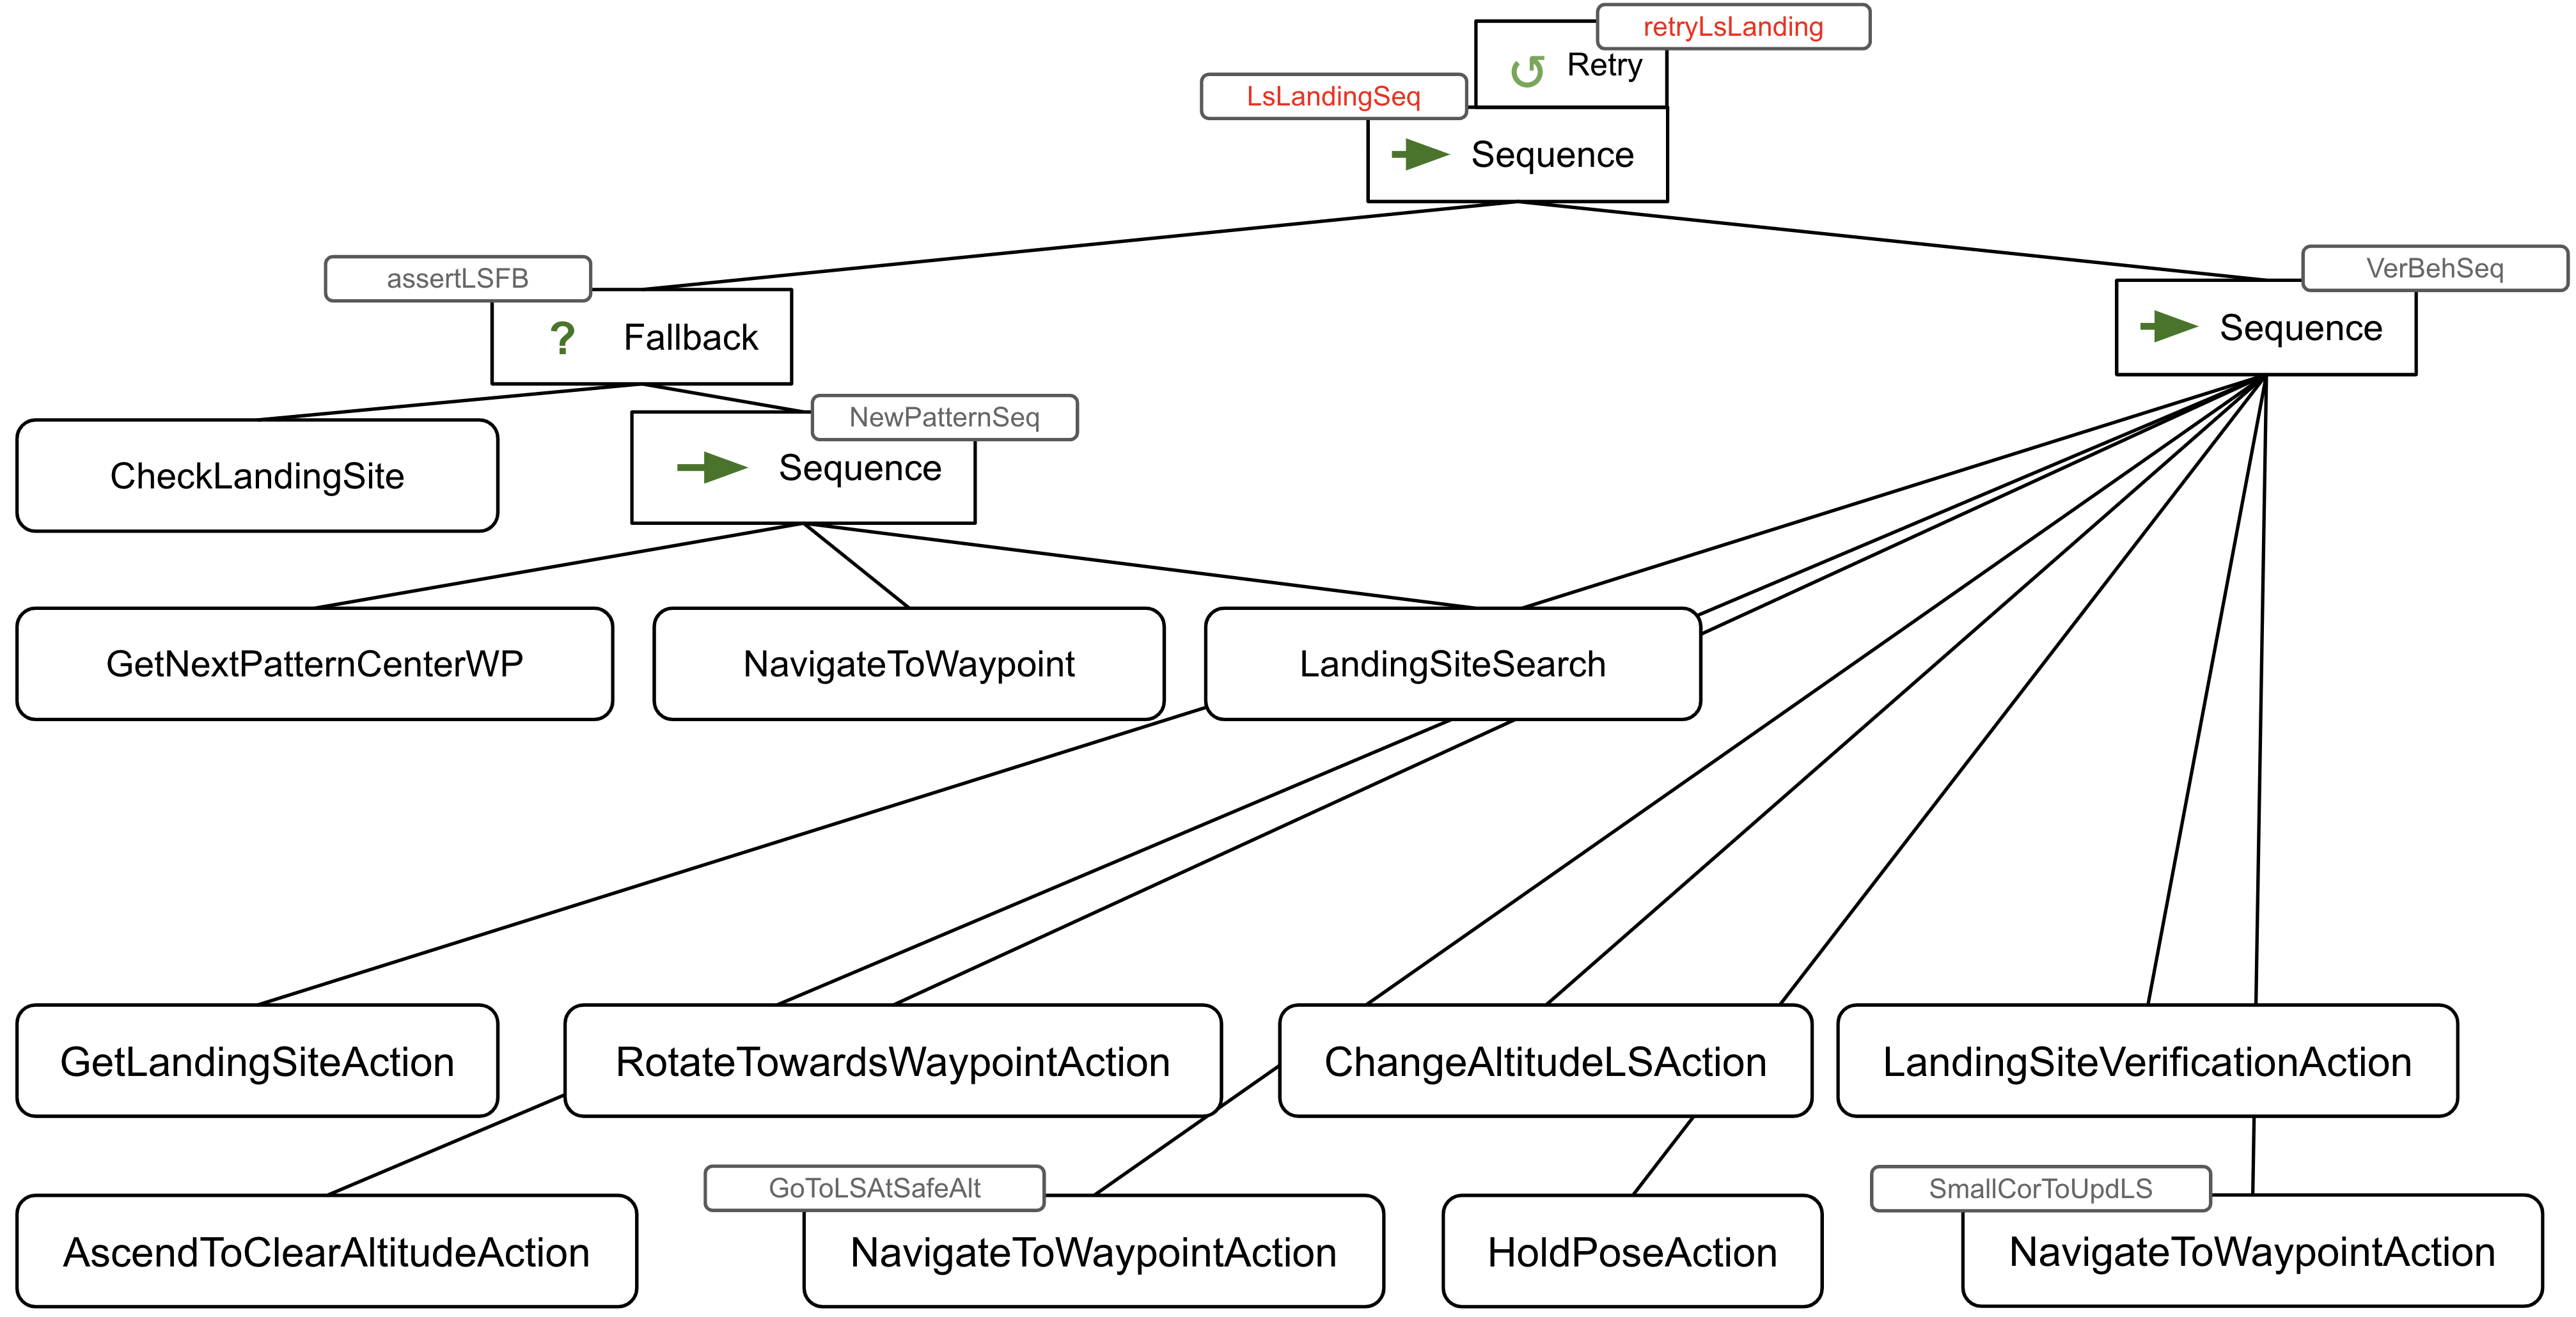
\includegraphics[scale=0.18]{images/autonomous_landing/landing_behavior_BT.png}
\caption{Landing procedure implementation as behavior tree}
\label{fig:landing_BT}
\end{figure}

The left part summarized by the assertLSFB (aka assert landing site fallback) checks, whether landing sites were detected. If they were, the fallback yields success directly. Otherwise, a landing site detection pattern sequence is executed. This side is covered by numbers 1. a) and 1. b) of the conceptual behavior in \cref{sec:concept_beh}.

The right side contains the behavior to be executed when a landing site has been found. These are exactly the steps laid out in numbers 2 - 6. b).


\subsubsection{Behavior to Land at Home Position}

The last behavior to define, though simpler than the previous, is the process of returning to and landing at the home position. 

The implementation thereof is shown in \cref{fig:bt_land_at_home}.

\begin{figure}[h]
\centering
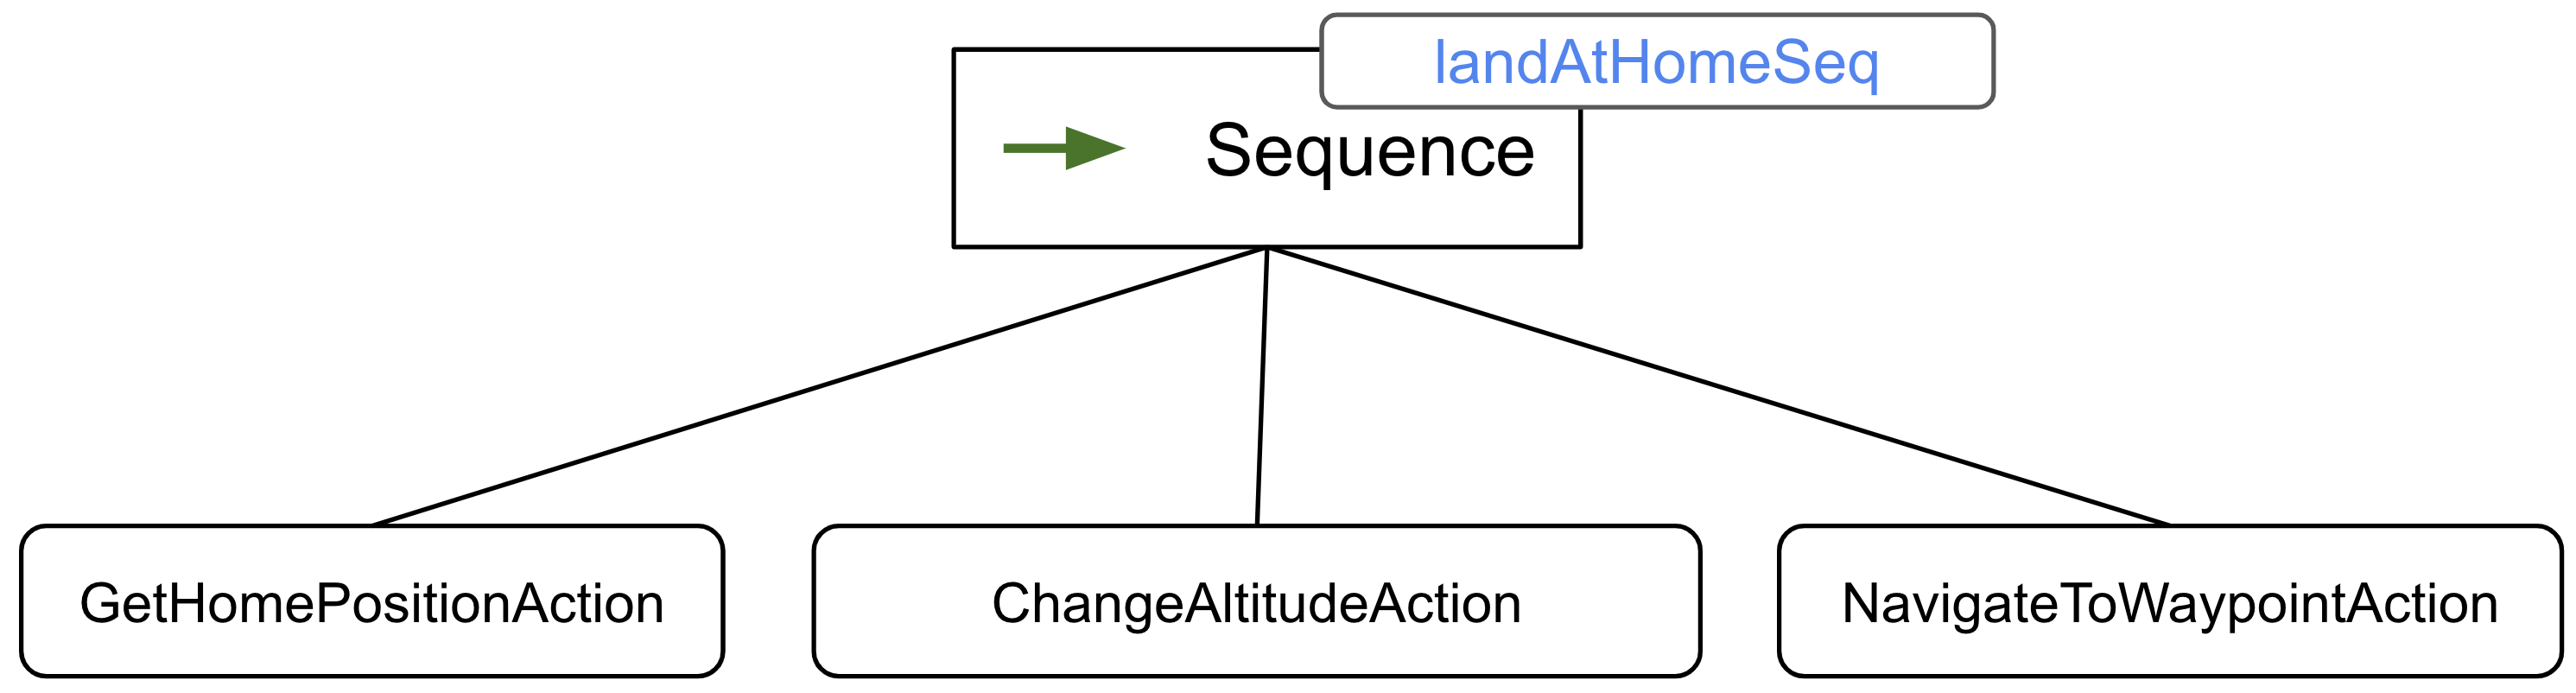
\includegraphics[scale=0.2]{images/autonomous_landing/land_at_home_beh.png}
\caption{Behavior tree of the implementation when landing at the home position}
\label{fig:bt_land_at_home}
\end{figure}

The behavior when landing at the home position is very similar to the landing site based landing, however, a bit simpler. The landing location is queried following which the drone ascends to a safe altitude and traverses to the home position. There, the landing action is then initiated.

\subsection{Full Pipeline in Action}

In the following, a simulated flight demonstrating this landing behavior is shown. \cref{fig:demo_flight_setup} shows the setup of the demonstration flight on the Arroyo map introduced in \cref{sec:simulation}. The drone takes off to 100 m altitude and traverses to the indicated location where the landing behavior is initiated.

\begin{figure}[h]
\centering
\includegraphics[scale=0.15]{images/autonomous_landing/flight_overview.png}
\caption{Demonstration flight setup: Left: Arroyo Seco Gazebo map, Right: QGroundControl mission to be flown at 100 m altitude}
\label{fig:demo_flight_setup}
\end{figure}

\subsubsection{Takeoff}

\begin{figure}[h]
\centering
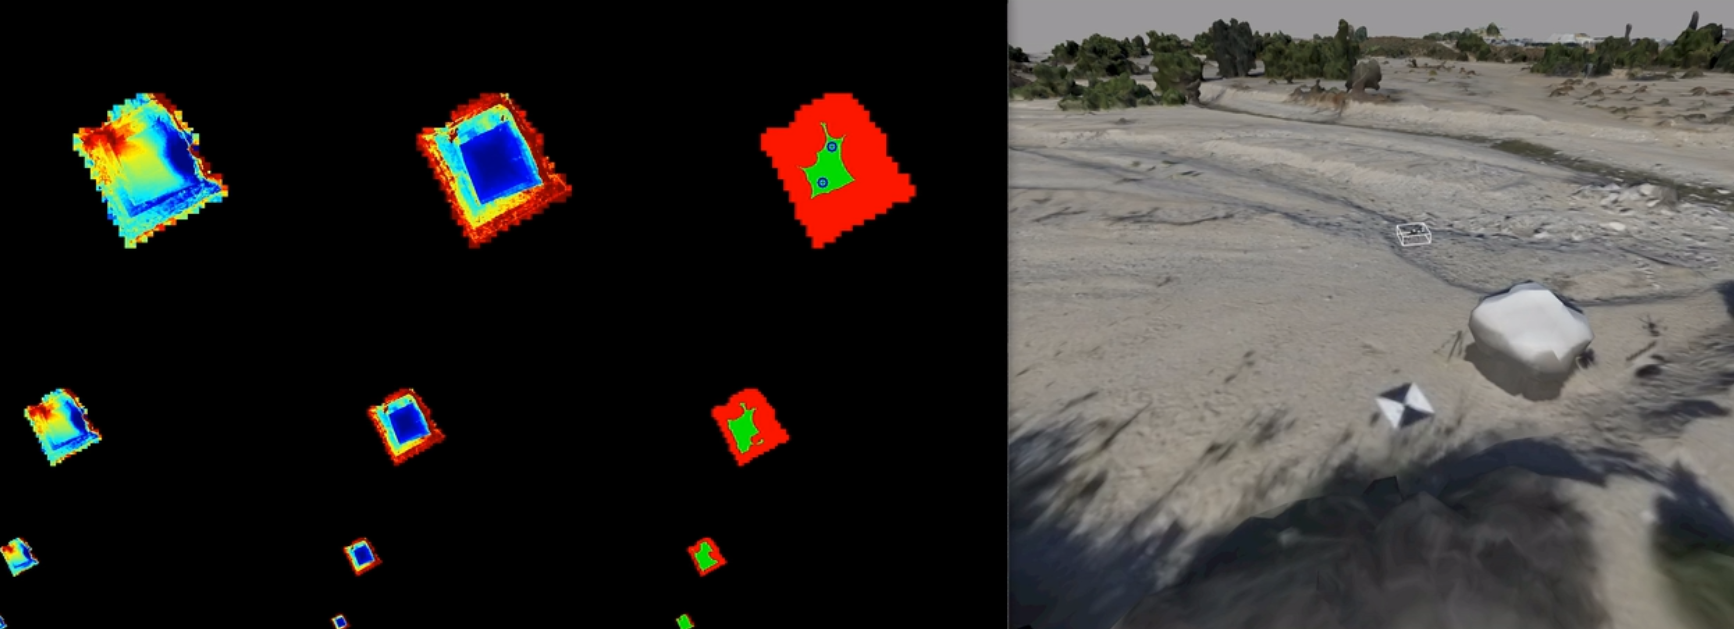
\includegraphics[scale=0.27]{images/autonomous_landing/demo_flight/takeoff1.png}
\caption{Takeoff of the drone: Left: LSD debug image, Right: Ascending drone in the simulation}
\label{fig:demo_takeoff1}
\end{figure}

\cref{fig:demo_takeoff1} shows the drone's takeoff. During this time LSD is supplied with stereo camera depth point clouds. Note the increasing uncertainty of the outer edges due to the increasing altitude and the fixed baseline.

\begin{figure}[h]
\centering
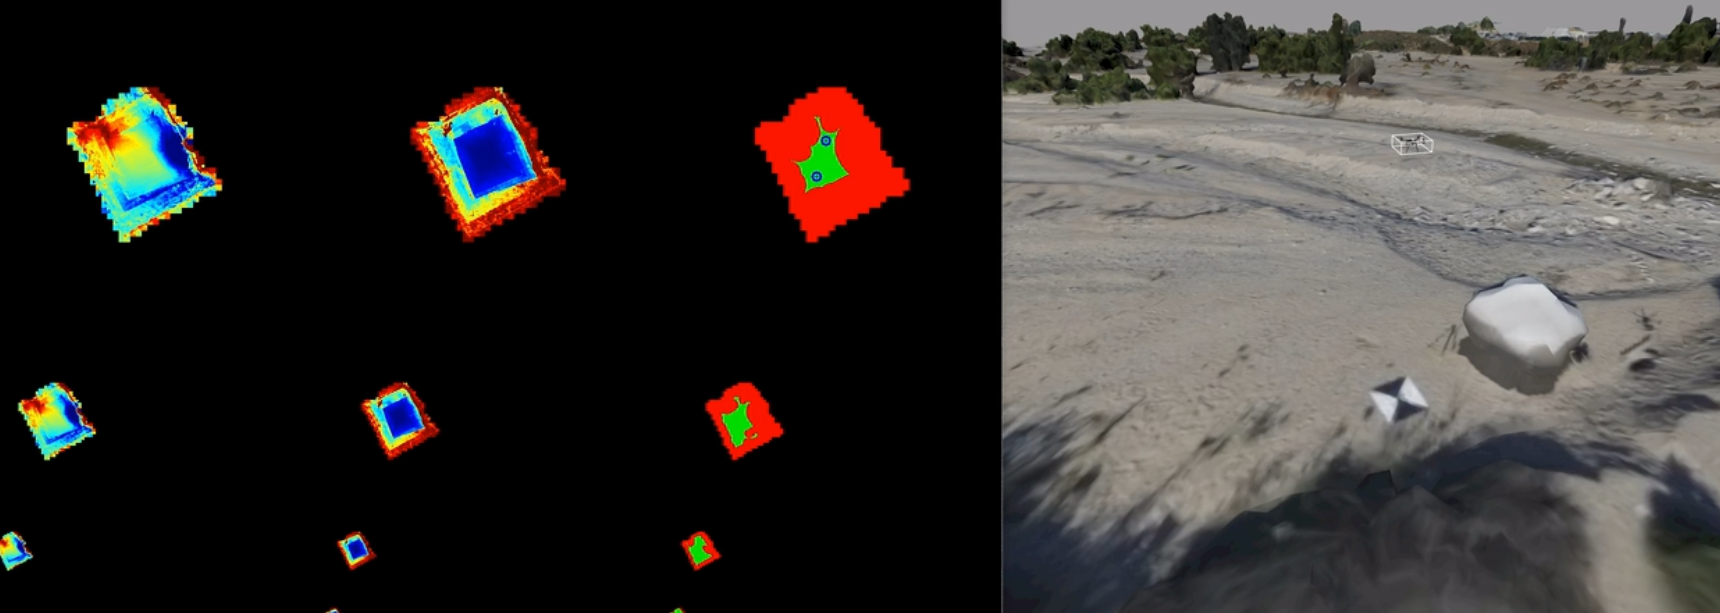
\includegraphics[scale=0.27]{images/autonomous_landing/demo_flight/takeoff2.png}
\caption{Later point of the drone's takeoff}
\label{fig:demo_takeoff2}
\end{figure}

\cref{fig:demo_takeoff2} shows the same takeoff at a later point in time. Note how the LSD debug image stayed the same despite the drone having risen to a higher altitude. This is because the stereo camera depth node has been switched off by the laser range finder readings and SFM took over. As SFM does not perceive depth during vertical ascent however, LSD does not register any input.

\subsubsection{Mission}

Upon reaching the cruise altitude, the first mission waypoint is pursued. The lateral motion allows SFM to slowly merge its information into the LSD DEM. After a few seconds the SFM information converges sufficiently in order for landing site to be detected on them. This is shown in \cref{fig:demo_mission1}.

\begin{figure}[h]
\centering
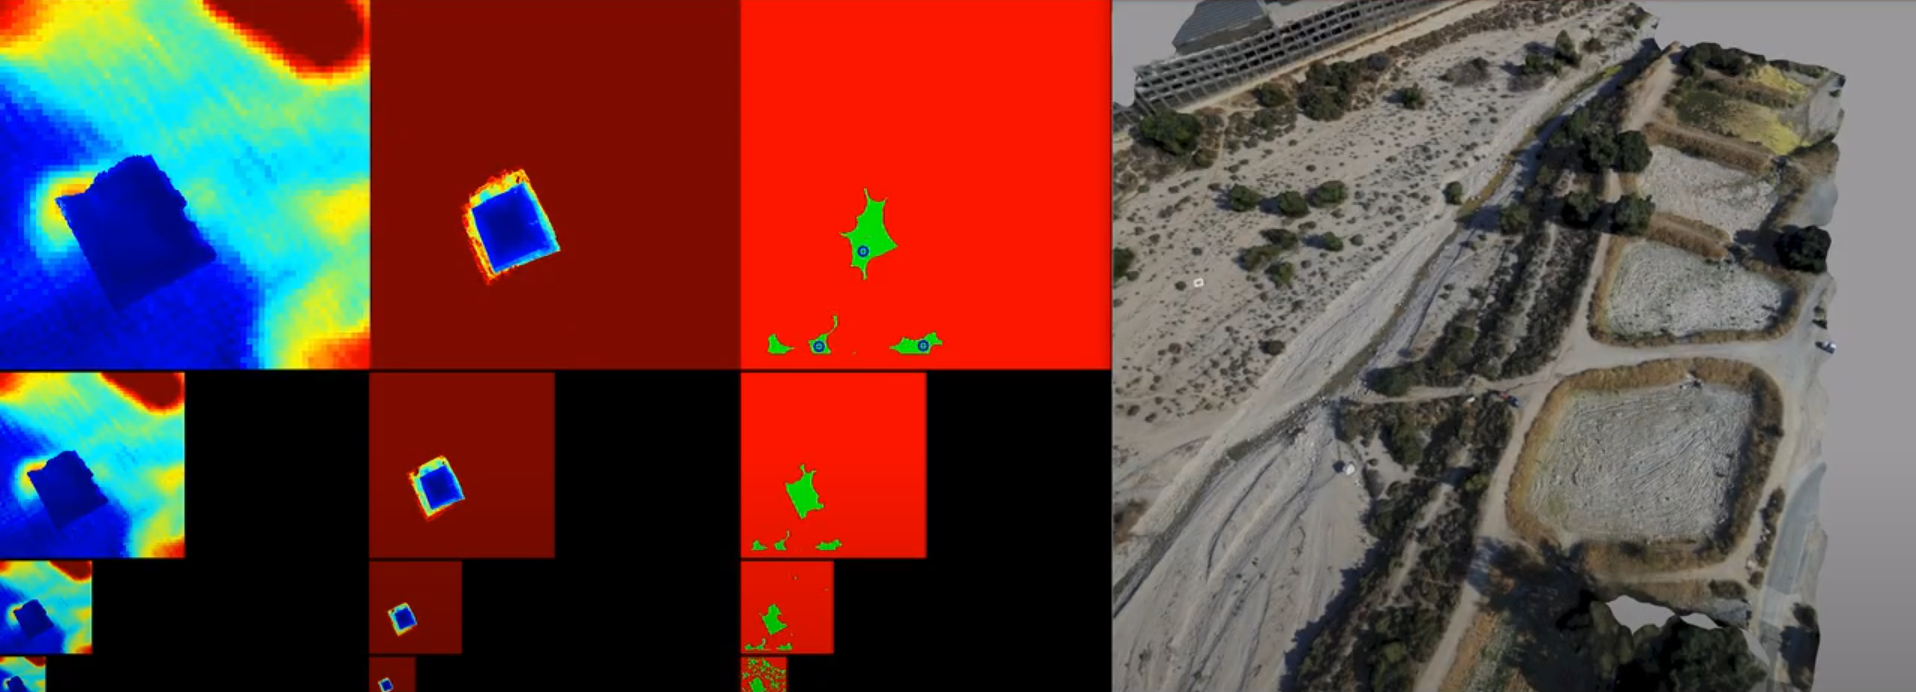
\includegraphics[scale=0.25]{images/autonomous_landing/demo_flight/mission1.png}
\caption{Initial traversal in the mission state upon reaching cruise altitude.}
\label{fig:demo_mission1}
\end{figure}

From this point onwards, the whole mission is flown with the SFM pipeline supplying LSD with depth information and LSD sending detected landing sites to the autonomy.

When reaching the last waypoint of the mission, the landing state is initiated. 

\begin{figure}[h]
\centering
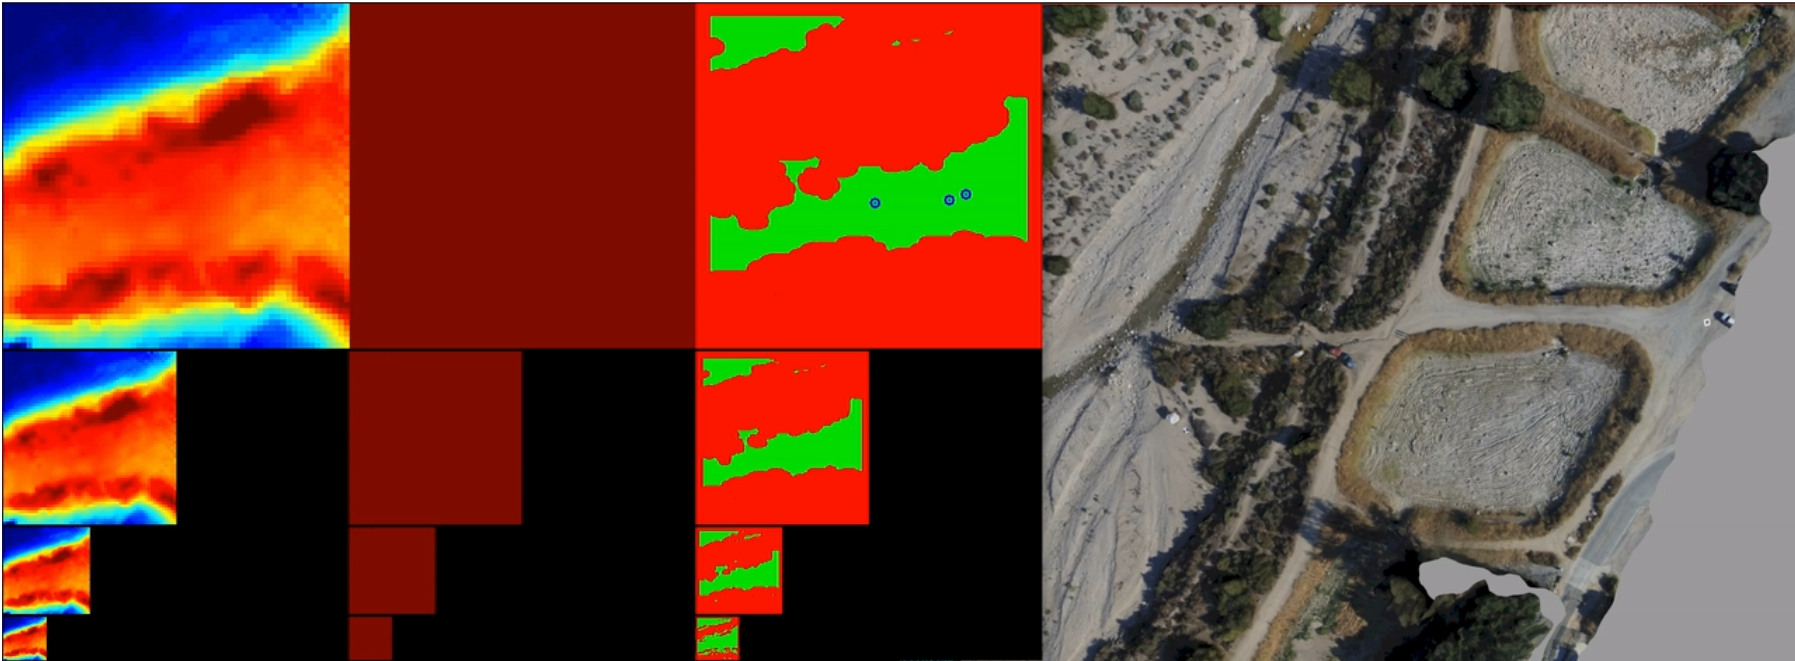
\includegraphics[scale=0.25]{images/autonomous_landing/demo_flight/mission_end.png}
\caption{End of mission state}
\label{fig:demo_mission_end}%TODO replace with SFM images
\end{figure}

\clearpage %HERE
\subsubsection{Landing Behavior}

Following the landing procedure visualized in \cref{fig:landing_BT}, a landing site is selected. 

\begin{figure}[h]
\centering
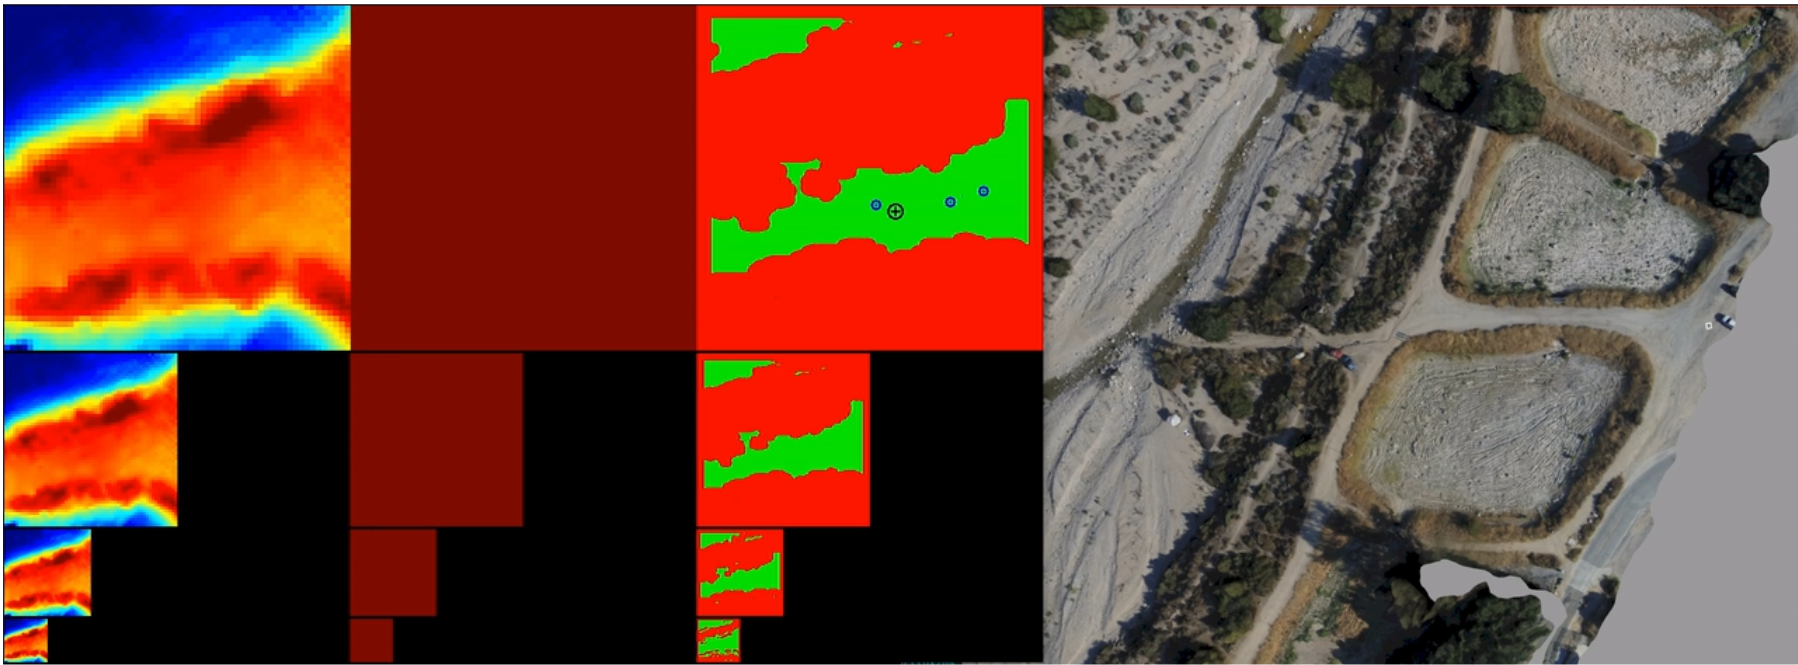
\includegraphics[scale=0.25]{images/autonomous_landing/demo_flight/ls_selection.png}
\caption{Start of landing sequence: the best landing site is selected and indicated in the LSD debug window with the black encircled cross.}
\label{fig:demo_ls_selection}
\end{figure}

Following the outlined behavior, the drone ascends to a clear altitude and traverses to the landing site location, where it descends to a verification altitude above the ground. This is shown in \cref{fig:demo_ver}.

\begin{figure}[h]
\centering
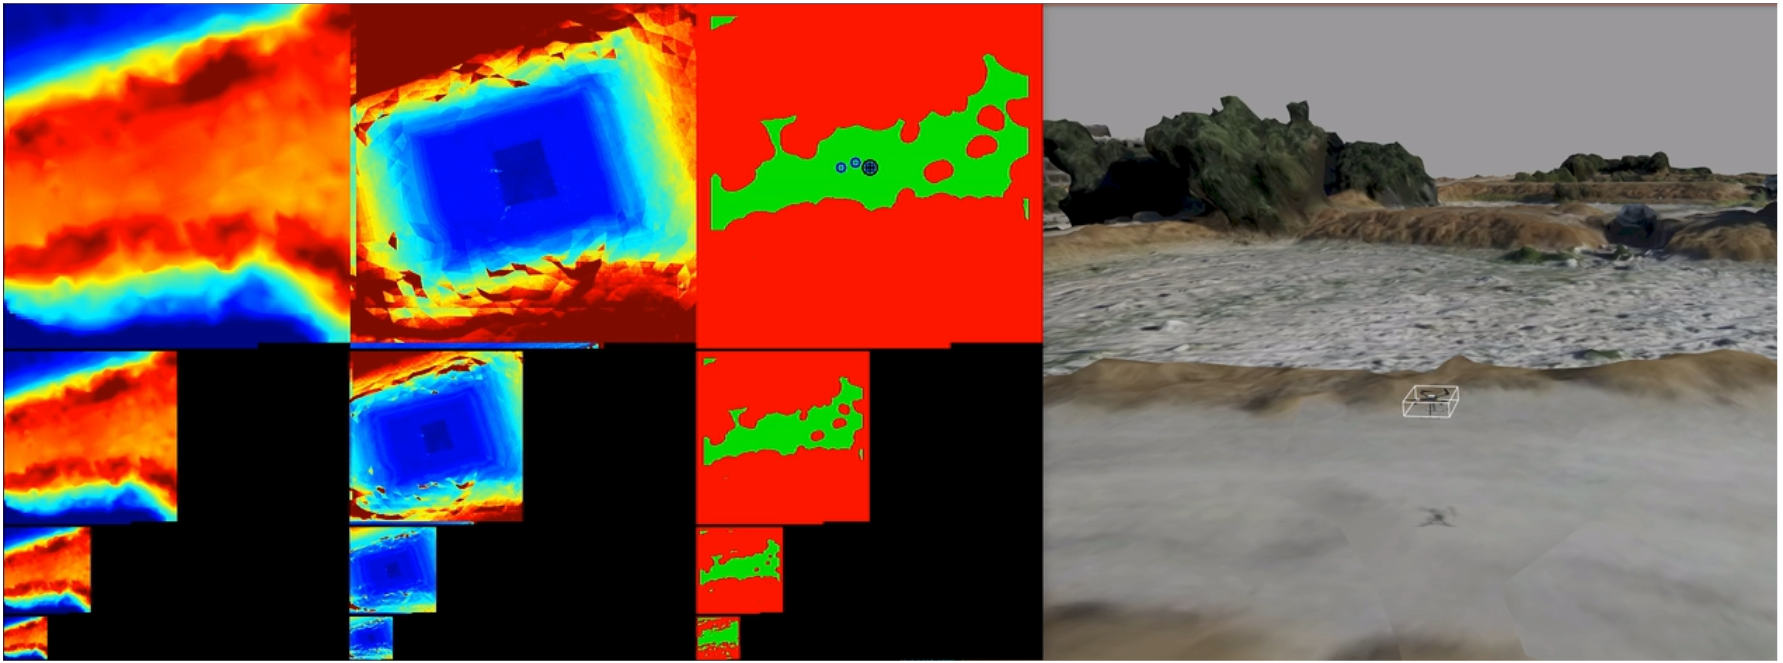
\includegraphics[scale=0.25]{images/autonomous_landing/demo_flight/verification.png}
\caption{Rotorcraft hovering on top of landing site and trying to re-detect chosen landing site}
\label{fig:demo_ver}
\end{figure}

Upon having verified the landing site in question, the last small re-detection correction of the landing site's position is considered and the drone adjusts accordingly as shown in \cref{fig:demo_last_correction}.

\begin{figure}[h]
\centering
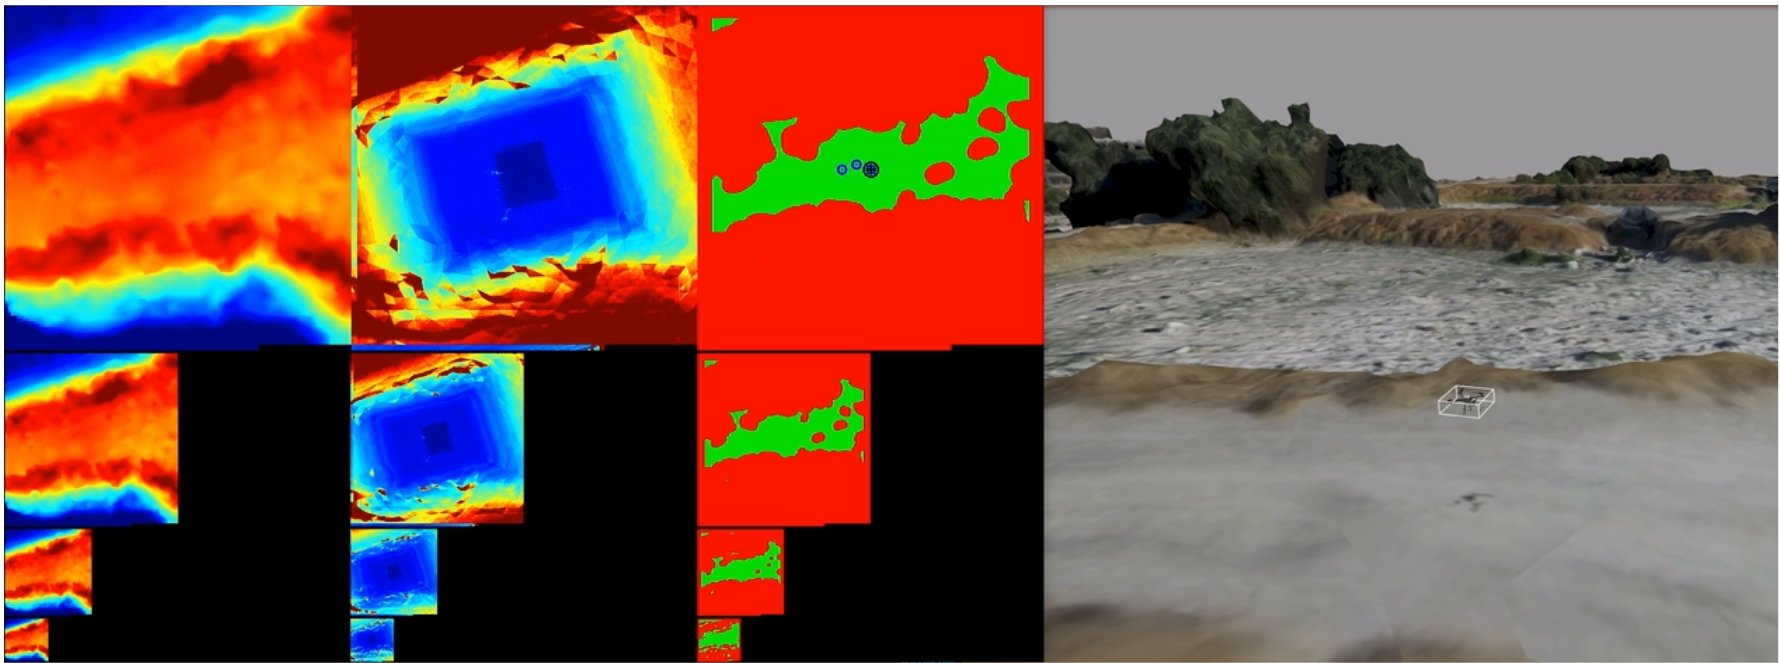
\includegraphics[scale=0.25]{images/autonomous_landing/demo_flight/last_correction.png}
\caption{Rotorcraft adjusts position to refined landing site location}
\label{fig:demo_last_correction}
\end{figure}

\subsubsection{Final Landing Action}

Finally, the drone can land safely. It descends with a constant velocity which is decreased upon entering a minimum proximity to the landing altitude.
\cref{fig:demo_final_landing} shows the final location of the rotorcraft after the landing procedure.

\begin{figure}[h]
\centering
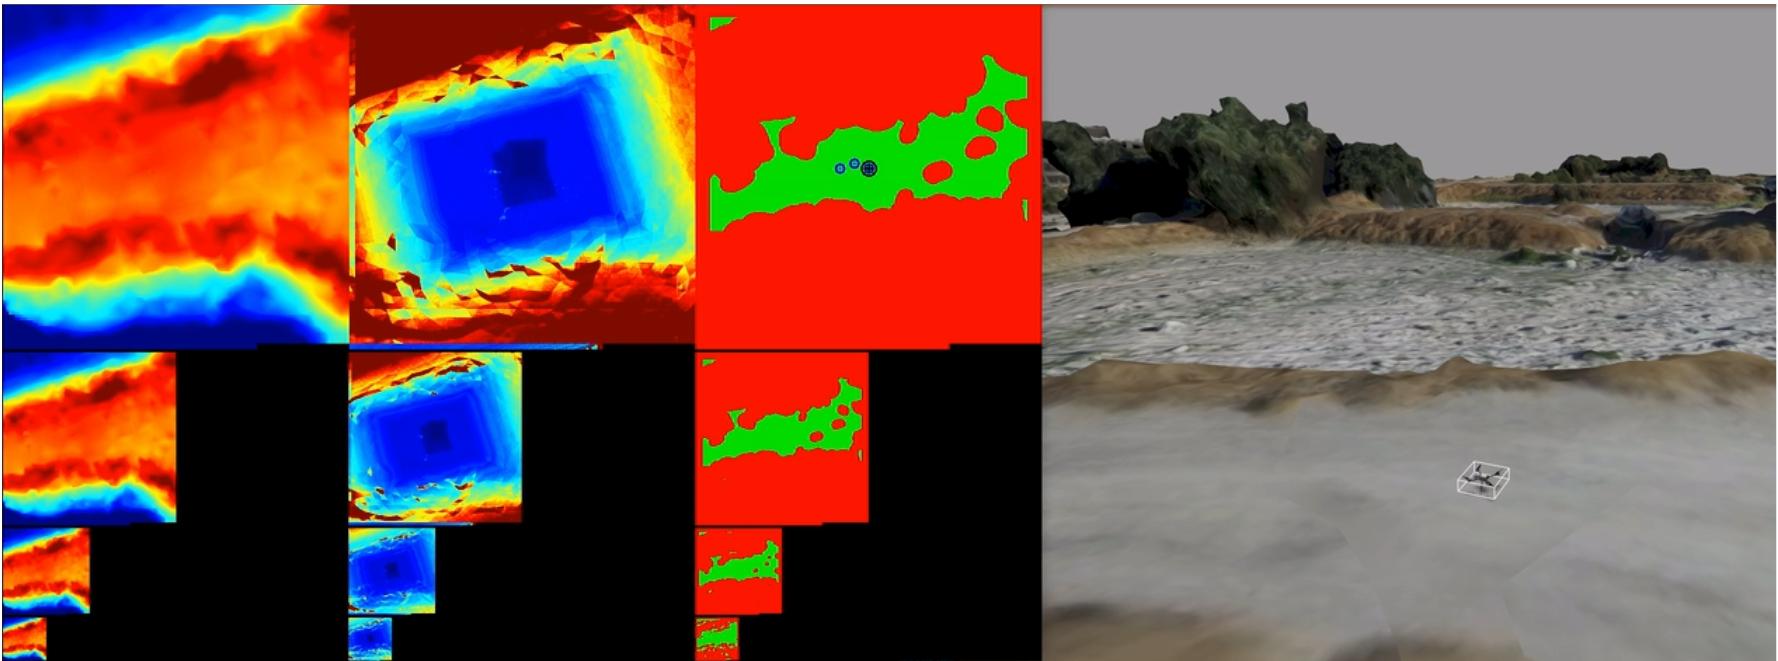
\includegraphics[scale=0.25]{images/autonomous_landing/demo_flight/landed.png}
\caption{Final landing of the drone chosen by LSD}
\label{fig:demo_final_landing}
\end{figure}







